% -*- coding: utf-8 -*-
\documentclass[UTF8,a4paper,10pt,fontset=windows]{ctexart}
\usepackage[left=3.17cm, right=3.17cm, top=2.74cm, bottom=2.74cm]{geometry}
\usepackage{amsmath}
\usepackage{amssymb}
\usepackage{graphicx}
\usepackage{float}
\usepackage{cite}
\usepackage{caption}
\usepackage{booktabs}
\usepackage{multirow}
\usepackage{array}
\usepackage{xcolor}
\usepackage{listings}
\usepackage[colorlinks,linkcolor=black,anchorcolor=blue,citecolor=black,urlcolor=blue]{hyperref}
\usepackage{fancyhdr}
\usepackage{algorithm}
\usepackage{algorithmicx}
\usepackage{algpseudocode}

\pagestyle{fancy}
\lhead{\kaishu \leftmark}
\rhead{\kaishu 并行程序设计实验报告}
\cfoot{\thepage}
\renewcommand{\headrulewidth}{0.1pt}
\renewcommand{\footrulewidth}{0pt}
\newcommand{\HRule}{\rule{\linewidth}{0.5mm}}

\lstset{
  breaklines=true,
  basicstyle=\small\ttfamily,
  keywordstyle=\color{blue!70}\bfseries,
  commentstyle=\color{red!50!green!50!blue!50},
  stringstyle=\ttfamily,
  numbers=left,
  numberstyle=\tiny\color{blue!50},
  frame=trbl
}

\floatname{algorithm}{Algorithm}
\renewcommand{\algorithmicrequire}{\textbf{Input:}}
\renewcommand{\algorithmicensure}{\textbf{Output:}}

\begin{document}

\begin{titlepage}
    \begin{center}
    
\includegraphics[width=0.8\textwidth]{NKU.png}\\[1cm]
    \textsc{\Huge \kaishu{\textbf{南\ \ \ \ \ \ 开\ \ \ \ \ \ 大\ \ \ \ \ \ 学}} }\\[0.9cm]
    \textsc{\huge \kaishu{\textbf{计\ \ 算\ \ 机\ \ 学\ \ 院}}}\\[0.5cm]
    \textsc{\Large \textbf{并行程序设计期末实验报告}}\\[0.8cm]
    \HRule \\[0.9cm]
    { \LARGE \bfseries 基于 MPI 任务池的矩阵 SVD 算子并行化实验}\\[0.4cm]
    \HRule \\[2.0cm]
    \centering
    \textsc{\LARGE \kaishu{姓名\ :\ 邹俊轩}}\\[0.5cm]
    \textsc{\LARGE \kaishu{学号\ :\ 2412592}}\\[0.5cm]
    \textsc{\LARGE \kaishu{年级\ :\ 2024级}}\\[0.5cm]
    \textsc{\LARGE \kaishu{专业\ :\ 计算机科学与技术}}\\[0.5cm]
    \textsc{\LARGE \kaishu{指导教师\ :\ 王刚}}\\[0.5cm]
    \textsc{\Large \kaishu{GitHub 仓库\ :\ \href{https://github.com/pointzu/mpi}{https://github.com/pointzu/mpi}}}\\[0.5cm]
    \vfill
    {\Large \today}
    \end{center}
\end{titlepage}

\newpage
\thispagestyle{empty}
\renewcommand{\abstractname}{\kaishu \large \textbf{摘要}}
\begin{abstract}
本实验选择矩阵奇异值分解（SVD）算子作为 MPI 编程题目。将并行化集中在 Golub-Kahan（GKH）迭代阶段：0 号进程负责维护活动块任务池，其余进程空闲后领取非平凡活动块，执行一轮 bulge chasing，并只回传对应的 $B$ 子块以及 $U,V$ 的相关列。实验在课程服务器上采用 \texttt{mpic++} 编译并通过 \texttt{qsub\_mpi.sh} 提交，共采集 41 组有效运行数据，覆盖 MPI 进程数、编译优化等级、SIMD 开关和重复运行稳定性。全部原始输出均通过 5 个测试样例，最大相对重构误差为 $4.80\times10^{-13}$，最大正交误差约为 $2.38\times10^{-13}$。

实验表明，普通随机矩阵上的 SVD 并不随 MPI 进程数单调加速。以 GKH 阶段为例，$np=4$ 时平均耗时从 $23147.60$ ms 降至 $15975.63$ ms，加速比为 1.45；继续增加到 $np=8$、$np=16$ 后收益下降，$np=32$ 反而退化为 0.34 倍。主要原因是 GKH 的活动块并行度不足，且跨节点通信、矩阵广播和结果合并开销快速增大。SIMD 对上二对角化阶段有 1.26 倍收益，但在 MPI+GKH 阶段几乎没有改善，说明此时瓶颈已经由向量计算转向任务粒度和通信开销。本文据此给出基于实验数据的性能分析和后续改进方向。

\noindent\textbf{关键词：} SVD；MPI；Golub-Kahan；任务池；SIMD；性能分析
\end{abstract}

\tableofcontents
\newpage
\setcounter{page}{1}

\section{实验目标与要求理解}

\subsection{选题要求}
SVD 章节指出，多进程版本的难点在于：各进程地址空间独立，矩阵拷贝和通信开销很大，结果合并时竞争更严重，

手册对 SVD 提出了三个重点：第一，实现主从式结构，至少完成一个任务池；第二，围绕子矩阵或活动块组织迭代，避免已经收敛的 $1\times1$ 子问题反复参与计算；第三，完成加速和 profiling。

\subsection{完成内容概述}
本次实验在上一次 SVD 代码基础上完成如下工作：

\begin{itemize}
  \item 在 \texttt{matrix.h} 中增加连续内存访问接口，使 MPI 能够广播矩阵数据。
  \item 在 \texttt{gkh.cpp} 中加入 \texttt{SVD\_USE\_MPI} 条件编译路径；使用 MPI 编译时，GKH 阶段默认进入 MPI 任务池模式。
  \item 设计 0 号进程调度、其他进程工作领取的主从式活动块任务池。只将长度大于 1 的非平凡活动块放入任务池，已经收敛的 $1\times1$ 块不再生成计算任务。
  \item 继承前序实验中的 SIMD 优化路径，并通过 \texttt{-DSVD\_DISABLE\_SIMD} 做对比实验。
\end{itemize}


\section{算法与 MPI 并行设计}

\subsection{串行 SVD 流程}
程序对 $m\times n$ 矩阵 $A$ 计算 SVD。第一阶段使用左右 Householder 变换将矩阵化为上二对角矩阵：
\[
    A = U B V^T .
\]
第二阶段在上二对角矩阵 $B$ 上执行 Golub-Kahan 迭代，通过 Wilkinson shift 和 Givens 旋转进行 bulge chasing，使超对角元素逐步收敛到 0。最后程序将奇异值调整为非负并降序排列，得到标准化的 $S$ 矩阵。该流程来自经典 SVD 算法\cite{golub1965calculating,golub1970singular}。

\subsection{活动块并行粒度}
GKH 迭代中，如果某个超对角元素已经足够接近 0，则上二对角矩阵可以被切分为多个相互独立的活动块。一个活动块 $[l,r]$ 表示第 $l$ 到第 $r$ 个奇异值相关的子问题尚未收敛。不同活动块之间不共享 $B$ 的子块，更新 $U,V$ 时也只涉及不重叠的列区间，因此可以在同一轮中并行处理。

不过，普通随机矩阵通常会在较长时间内保持一个大的活动块。此时即便启动多个 MPI 进程，也只有一个块可以推进，其余进程只能等待。只有当 deflation 产生多个非平凡活动块，或者输入矩阵本身具有块结构时，活动块任务池才有足够并行度。因此本实验的核心问题不是“MPI 是否一定加速”，而是通过数据判断：在本框架的端到端 SVD 测试中，活动块并行度是否足以抵消通信和复制开销。

\subsection{主从式任务池}
本实现采用 0 号进程作为调度者，其他进程作为工作进程。根进程扫描当前上二对角矩阵，将非平凡活动块按工作量排序后放入任务池。若任务数为 0，说明 GKH 已收敛；若任务数为 1，则根进程直接串行执行，避免把完整矩阵广播给其他进程却没有可用并行度；若任务数大于 1，则根进程广播当前 $U,B,V$，工作进程领取活动块并执行一轮 bulge chasing。

\begin{algorithm}[H]
\caption{MPI-GKH 活动块任务池}
\begin{algorithmic}[1]
\Require 当前 $U,B,V$，最大迭代次数 \texttt{max\_iter}，容忍误差 \texttt{tol}
\Ensure 收敛后的 $U,S,V$
\For{$iter=1$ to \texttt{max\_iter}}
  \State 0 号进程清理数值噪声，并按超对角元素切分活动块
  \State 将长度大于 1 的非平凡活动块放入任务池
  \If{任务池为空}
    \State 广播停止命令，进入最终标准化
  \ElsIf{任务池只有一个活动块}
    \State 0 号进程本地执行该活动块，其他进程等待下一轮命令
  \Else
    \State 0 号进程广播当前 $U,B,V$
    \State 工作进程领取活动块并执行一轮 bulge chasing
    \State 工作进程回传 $B[l:r,l:r]$、$U[:,l:r]$、$V[:,l:r]$
    \State 0 号进程合并互不重叠的局部结果
  \EndIf
\EndFor
\State 0 号进程将奇异值非负化并降序排序
\end{algorithmic}
\end{algorithm}

该设计没有强行并行化单个活动块内部的 Givens 旋转序列，因为 bulge chasing 本身存在顺序依赖。实验也会看到，进程数超过活动块并行度后，更多 MPI 进程不会自动带来加速。

\subsection{通信量设计}
在需要并行分发任务的一轮中，根进程广播完整的 $U,B,V$，使所有工作进程从一致状态开始。工作进程完成活动块后不回传完整矩阵，而只回传：
\[
    B[l:r,l:r],\quad U[:,l:r],\quad V[:,l:r].
\]
若活动块长度为 $k$，矩阵规模近似为 $n\times n$，回传 double 数量约为 $k^2+2nk$。当活动块较小时，该策略比回传完整矩阵明显更省；当只有一个大块时，本实现退回根进程串行处理，避免没有并行收益的全矩阵广播。

\section{实现与代码分析}

\subsection{文件结构}
表\ref{tab:files} 给出本次实验涉及的主要文件。本报告关注算法、代码结构、实验数据和分析.

\begin{table}[H]
\centering
\begin{tabular}{p{0.27\textwidth}p{0.63\textwidth}}
\toprule
文件 & 作用 \\
\midrule
\texttt{matrix.h} & 矩阵存储与基础运算。本次增加 \texttt{data()} 和 \texttt{size()}，用于 MPI 广播连续内存。\\
\texttt{bidiagonalization.cpp} & Householder 上二对角化，保留前序 SIMD 优化。\\
\texttt{gkh.cpp} & Golub-Kahan 迭代。本次新增 MPI 活动块任务池，并保留 serial、pthread、OpenMP 路径。\\
\texttt{qsub\_mpi.sh} & 按修正脚本说明提交 MPI 作业.\\
\bottomrule
\end{tabular}
\caption{实验主要文件}
\label{tab:files}
\end{table}

\subsection{矩阵连续内存接口}
MPI 的 \texttt{MPI\_Bcast} 只能广播连续缓冲区，因此原有矩阵类需要暴露底层连续数组。这里没有改变矩阵数据结构，只是在 \texttt{matrix.h} 中增加访问接口：

\begin{lstlisting}[language=C++]
double *data() { return data_.data(); }
const double *data() const { return data_.data(); }
int size() const { return rows_ * cols_; }
\end{lstlisting}

这一改动的作用比较基础，但很关键。若仍然通过逐行发送或逐元素发送矩阵，MPI 通信次数会大幅增加，且代码容易在 $U,B,V$ 三个矩阵同步时出错。使用连续内存后，矩阵广播只需要先广播维度，再广播 \texttt{double} 数组：

\begin{lstlisting}[language=C++]
int dims[2] = {M.rows(), M.cols()};
MPI_Bcast(dims, 2, MPI_INT, 0, MPI_COMM_WORLD);
MPI_Bcast(M.data(), M.size(), MPI_DOUBLE, 0, MPI_COMM_WORLD);
\end{lstlisting}

\subsection{模式选择}
MPI 模式选择放在 \texttt{gkh.cpp} 内部完成。程序读取环境变量 \texttt{SVD\_MODE}；如果显式设置为 \texttt{serial}、\texttt{pthread}、\texttt{openmp} 或 \texttt{mpi}，则按指定模式运行；若使用 \texttt{-DSVD\_USE\_MPI} 编译且没有设置环境变量，则默认进入 MPI 路径。

\begin{lstlisting}[language=C++]
#ifdef SVD_USE_MPI
return GkhMode::Mpi;
#else
return GkhMode::Pthread;
#endif
\end{lstlisting}

这样设计的好处是：同一份 \texttt{main.cpp} 可以在普通 C++ 编译和 MPI 编译之间复用；服务器上只需要改变编译命令，而不需要改测试入口。MPI 初始化也采用延迟初始化：当 GKH 第一次进入 MPI 路径时检查 \texttt{MPI\_Initialized}，若尚未初始化则由 \texttt{gkh.cpp} 调用 \texttt{MPI\_Init}，并通过 \texttt{atexit} 注册 \texttt{MPI\_Finalize}。此外，非 0 号进程会关闭 \texttt{std::cout}，避免所有 rank 重复输出测试结果。

\subsection{任务分发与工作进程协议}
MPI 部分使用三类命令控制工作进程：

\begin{itemize}
  \item \texttt{MPI\_CMD\_STOP}：GKH 已结束，工作进程退出循环；
  \item \texttt{MPI\_CMD\_IDLE\_SERIAL}：本轮只有一个非平凡活动块，由 0 号进程串行推进，工作进程等待；
  \item \texttt{MPI\_CMD\_DISTRIBUTE}：本轮存在多个活动块，广播矩阵并分发任务。
\end{itemize}

根进程在任务池中按工作量从大到小排序活动块，先给每个工作进程发送一个任务，自己也处理一个任务。随后根进程使用 \texttt{MPI\_ANY\_SOURCE} 接收完成结果，哪个进程先完成就继续给它分配下一个任务。这相当于 MPI 版的动态调度，能够缓解活动块大小不均造成的负载不均。

\begin{lstlisting}[language=C++]
MPI_Recv(header, 2, MPI_INT, MPI_ANY_SOURCE,
         MPI_TAG_RESULT_HEADER, MPI_COMM_WORLD, &status);
const int worker = status.MPI_SOURCE;
...
if (next_task < task_count) {
    send_mpi_task(worker, tasks[next_task++]);
} else {
    send_mpi_stop(worker);
}
\end{lstlisting}

这一协议也是后续实验结果的解释基础：当 ready task 很少时，动态调度没有足够任务可分，MPI 进程数再多也只能等待；当 ready task 较多时，任务池才有可能体现收益。

\subsection{结果打包与通信开销}
工作进程完成活动块 $[l,r]$ 后不回传完整矩阵，而是把必要结果打包为一段连续数组。打包顺序为：

\begin{enumerate}
  \item 活动块对应的 $B[l:r,l:r]$；
  \item $U$ 中第 $l$ 到第 $r$ 列；
  \item $V$ 中第 $l$ 到第 $r$ 列。
\end{enumerate}

对于长度为 $k$ 的活动块，回传数据量为
\[
    k^2 + mk + nk
\]
个 \texttt{double}。这比回传完整 $U,B,V$ 小得多，但前提是活动块足够小。另一方面，每次进入并行分发轮次前，根进程仍需广播完整 $U,B,V$，这是当前实现最主要的通信成本。该设计是正确性优先的折中：先保证所有工作进程从完全一致的矩阵状态出发，再通过局部回传降低合并成本。后续若要继续优化，最有价值的方向是减少广播范围，例如只同步当前活动块相关列，或让工作进程持有跨轮状态，避免每轮全量同步。

\subsection{统计字段与 profiling}
\texttt{GkhRunStats} 中保留了迭代次数、活动块数量、可并行轮次、最大 ready task、MPI 任务发送数、矩阵广播字节数和结果回传字节数等字段。结合本次服务器数据，可以确认主要瓶颈确实不在数值正确性，而在活动块并行度与 MPI 通信开销的平衡。

\section{实验方法}

\subsection{实验环境与数据采集}
数据来自课程服务器，编译器使用 \texttt{mpic++}，MPI 头文件路径显示为 \texttt{mpich-aarch64}。任务通过 PBS 的 \texttt{qsub} 提交，每个计算节点最多申请 8 个核心，最多使用 4 个节点。

\begin{lstlisting}[language=bash]
mpic++ -std=c++17 -O2 -DSVD_USE_MPI main.cpp bidiagonalization.cpp gkh.cpp -o main
qsub qsub_mpi.sh
\end{lstlisting}

实验固定随机种子为 2412592，采集了四类数据：MPI 规模扩展、编译优化等级、SIMD 开关、固定配置重复运行。所有结果均按类别保存为 \texttt{data/results/raw/**/test.o} 和 \texttt{test.e}，汇总表为 \texttt{data/results/summary.csv}。本报告基于 41 组有效运行数据进行统计，图中误差线为同组重复运行的标准差。

图表绘制使用 Python 对 \texttt{summary.csv} 做二次统计，并采用 \texttt{SciencePlots} 与 Matplotlib 生成。增加了误差线、关键点标注、堆叠时间构成和热力图汇总，便于直接观察最优进程数、负优化区间和不同优化手段的贡献。

MPI 初始化放在 \texttt{gkh.cpp} 的 GKH 入口中。每个 MPI 进程在进入 GKH 前都会执行一次主程序中的上二对角化阶段，\texttt{test.o} 中也会看到若干重复样例标题。真正的 MPI 并行优化对象是 GKH 阶段，所以本文在讨论规模扩展时以 GKH 时间为主，同时保留端到端总时间作为参考。

\subsection{Profiling 设计}
本文采用“服务器计时数据 + 本地热点采样”的方式完成分析。服务器端主要依据 41 组真实 PBS 运行输出中的上二对角化时间、GKH 时间、不同进程数下的均值和标准差。这样可以直接观察 MPI 进程数增加后，通信、复制、等待和任务粒度对端到端时间的影响。作为补充，本地使用 Intel VTune 对\texttt{main.cpp} 单进程入口做热点采样，用来判断子进程内部主要计算热点。


\section{实验结果与分析}

\subsection{正确性验证}
41 组数据全部显示 \texttt{通过: 5 / 5}，未出现 \texttt{FAIL} 或 \texttt{converged: no}。所有测试样例中，最大相对重构误差为 $4.80\times10^{-13}$，最大 $U$ 正交误差为 $2.35\times10^{-13}$，最大 $V$ 正交误差为 $2.38\times10^{-13}$。这说明 MPI 任务分发、局部结果合并和 SIMD 开关都没有破坏 SVD 数值正确性。

\begin{table}[H]
\centering
\begin{tabular}{lrrr}
\toprule
指标 & 最大值 & 典型量级 & 结论\\
\midrule
相对重构误差 $\|A-USV^T\|_F/(\|A\|_F+1)$ & $4.80\times10^{-13}$ & $10^{-13}$ & 通过\\
$\|U^TU-I\|_F$ & $2.35\times10^{-13}$ & $10^{-13}$ & 通过\\
$\|V^TV-I\|_F$ & $2.38\times10^{-13}$ & $10^{-13}$ & 通过\\
通过样例数 & 5/5 & 所有 41 组 & 通过\\
\bottomrule
\end{tabular}
\caption{正确性实验摘要}
\label{tab:correctness}
\end{table}

\subsection{MPI 规模扩展}
表\ref{tab:scaling-real} 与图\ref{fig:mpi-scaling-time} 展示了不同进程数下的平均耗时。GKH 阶段在 $np=4$ 时达到本组实验最好结果，平均耗时为 $15975.63$ ms，相对 $np=1$ 的 $23147.60$ ms 加速 1.45 倍；但是 $np=8$ 时回升至 $17322.33$ ms，$np=16$ 时进一步回升至 $19177.90$ ms，$np=32$ 时显著退化为 $67490.93$ ms。端到端总时间的最优点同样出现在 $np=4$，为 $22707.15$ ms，相对 $np=1$ 的 $27481.56$ ms 加速 1.21 倍。

\begin{table}[H]
\centering
\small
\begin{tabular}{rrrrrrrr}
\toprule
$np$ & nodes & ppn & 上二对角/ms & GKH/ms & 总时间/ms & GKH加速比 & GKH效率\\
\midrule
1 & 1 & 1 & 4333.96 & 23147.60 & 27481.56 & 1.00 & 100.0\%\\
2 & 1 & 2 & 6080.27 & 22535.20 & 28615.47 & 1.03 & 51.4\%\\
4 & 1 & 4 & 6731.51 & 15975.63 & 22707.15 & 1.45 & 36.2\%\\
8 & 1 & 8 & 8795.52 & 17322.33 & 26117.86 & 1.34 & 16.7\%\\
16 & 2 & 8 & 9580.87 & 19177.90 & 28758.77 & 1.21 & 7.5\%\\
32 & 4 & 8 & 9400.84 & 67490.93 & 76891.77 & 0.34 & 1.1\%\\
\bottomrule
\end{tabular}
\caption{MPI 规模扩展实验平均结果，固定种子 2412592，每组 3 次}
\label{tab:scaling-real}
\end{table}

\begin{figure}[H]
\centering
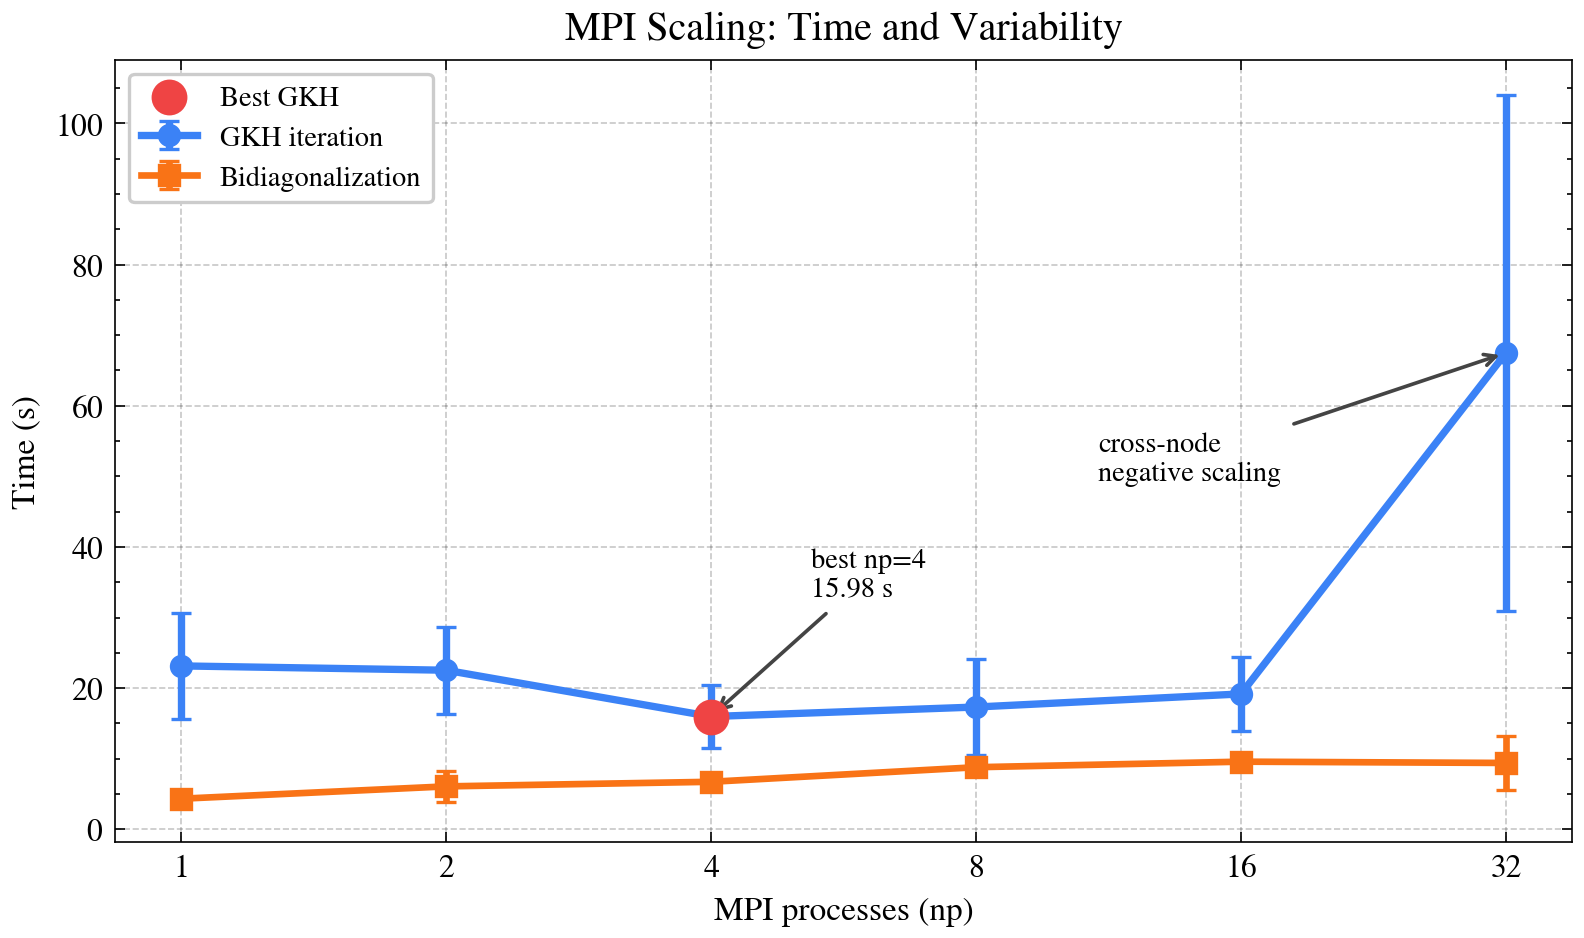
\includegraphics[width=0.78\textwidth]{figures/mpi_scaling_time.png}
\caption{MPI 规模扩展：上二对角化与 GKH 平均耗时}
\label{fig:mpi-scaling-time}
\end{figure}

\begin{figure}[H]
\centering
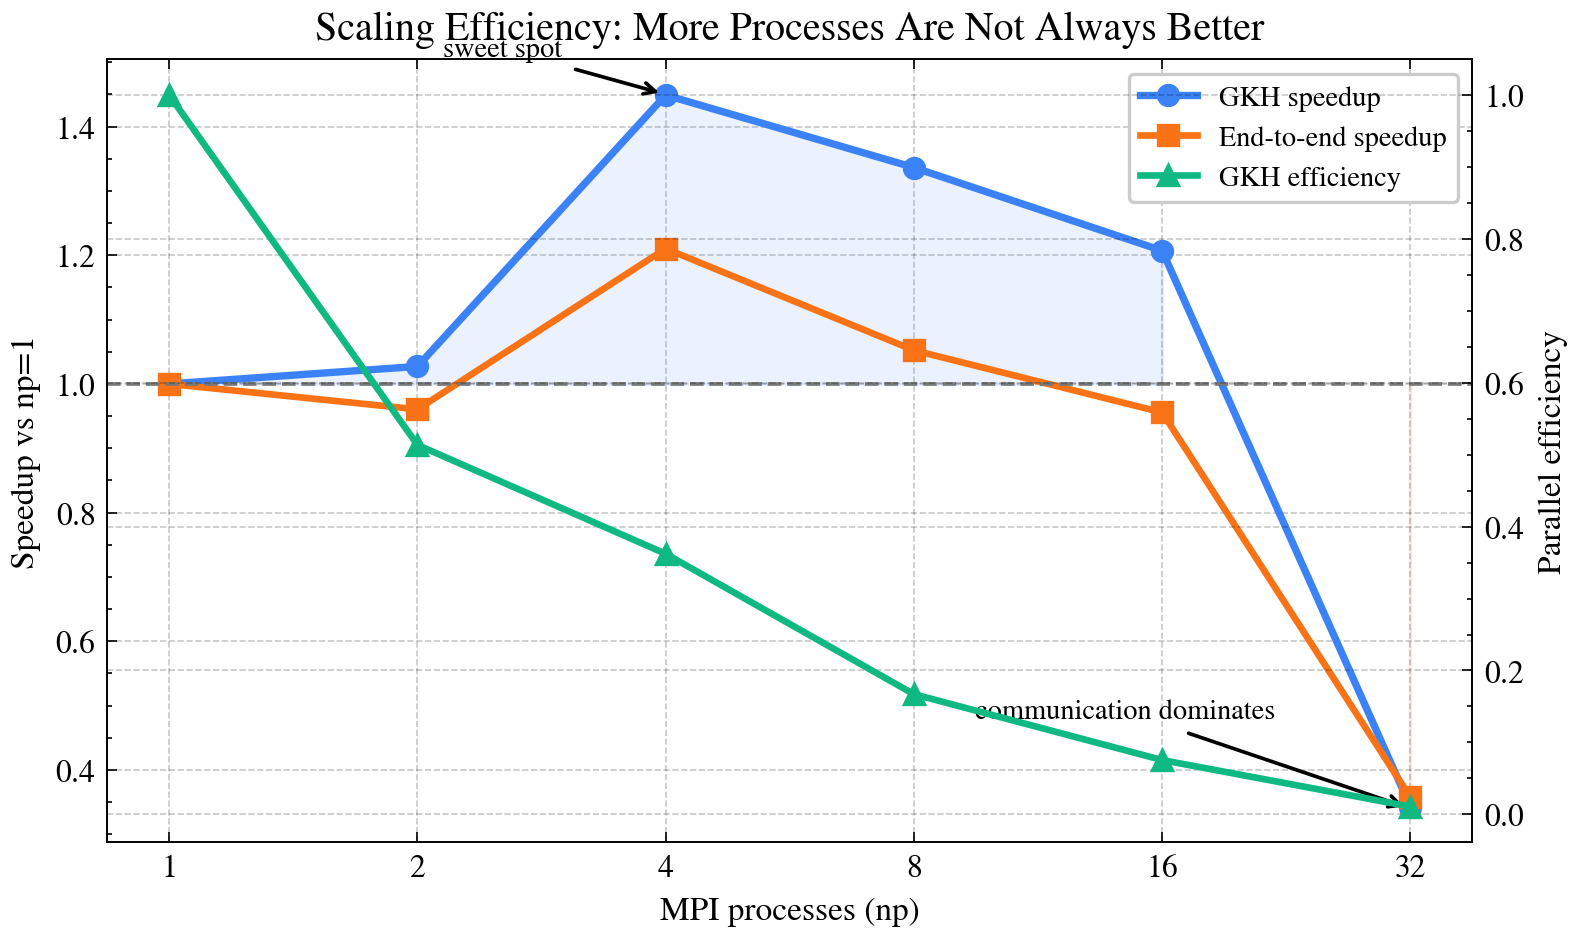
\includegraphics[width=0.78\textwidth]{figures/mpi_scaling_speedup.png}
\caption{MPI 规模扩展：加速比与并行效率}
\label{fig:mpi-scaling-speedup}
\end{figure}

图\ref{fig:mpi-heatmap} 用热力图汇总了同一组数据。所有行均为“越高越好”的指标，可以直观看出 $np=4$ 同时具有最高 GKH 加速比和最高端到端加速比，而 $np=32$ 在所有性能指标上都明显退化。尤其是 GKH 并行效率从 $np=4$ 的 36.2\% 下降到 $np=8$ 的 16.7\%、$np=16$ 的 7.5\%，到 $np=32$ 只剩 1.1\%。这表明瓶颈不是计算核心数量不足，而是可以被分发的有效任务太少。

\begin{figure}[H]
\centering
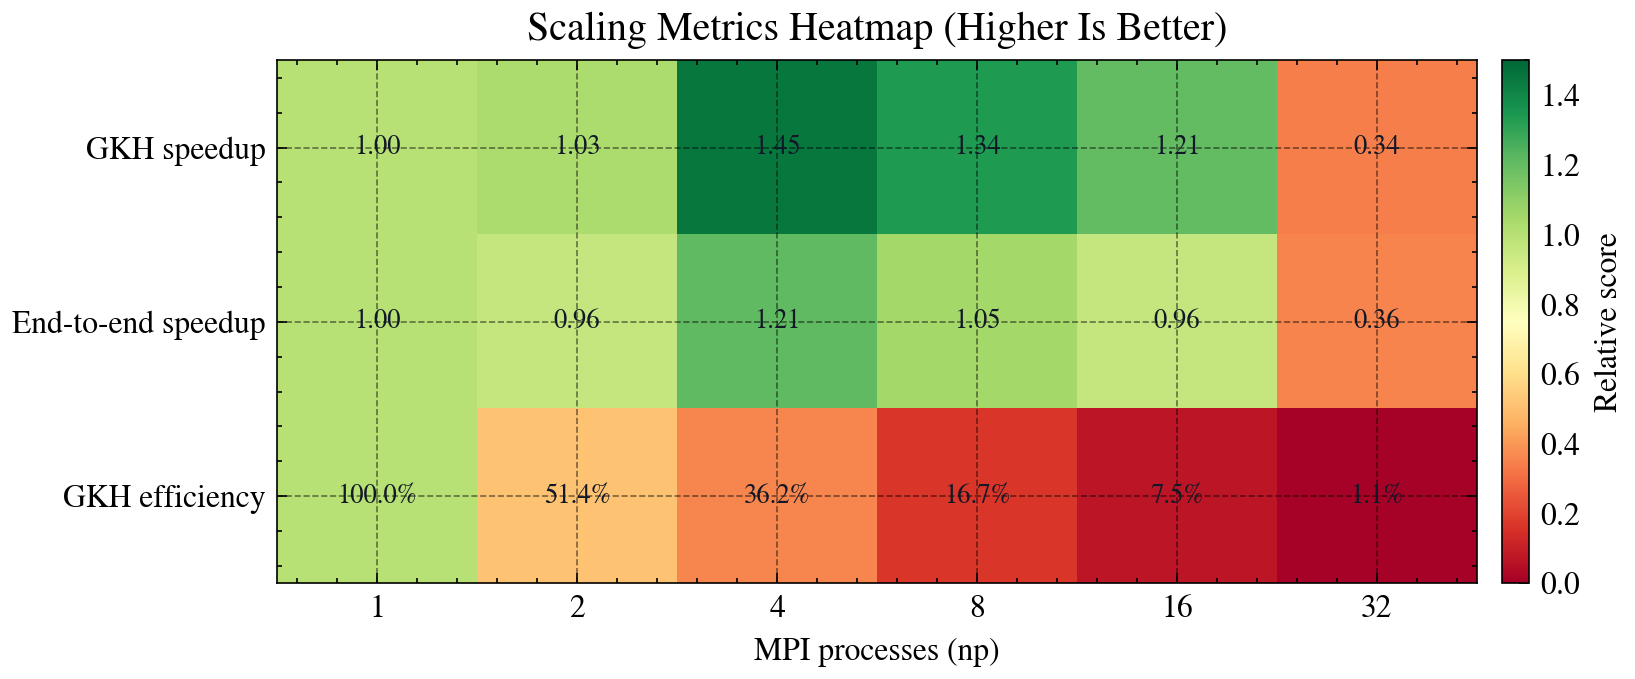
\includegraphics[width=0.82\textwidth]{figures/performance_heatmap.png}
\caption{规模扩展关键指标热力图}
\label{fig:mpi-heatmap}
\end{figure}

该结果说明，当前端到端随机矩阵测试中的可用活动块数量不足以支撑大量 MPI 进程。$np=2$ 只有 1.03 倍 GKH 加速，说明任务池已经被同步和调度开销明显抵消；$np=4$ 是较平衡点，仍在单节点内，通信成本较低；$np=16$ 进入跨节点后，广播 $U,B,V$ 和回收局部结果的代价上升；$np=32$ 虽满足脚本上限，但进程数远大于可同时处理的活动块数量，通信和等待成为主要开销，因此出现负优化。这也与实验手册中“大于 32 进程后通信时间会显著增长、加速意义不明显”的提示一致。

从数据波动看，$np=32$ 的 GKH 标准差约为 36.5 秒，明显高于其他组。这说明进程数过多不只是平均速度变慢，也会让运行稳定性变差。原因可能包括跨节点分配差异、每轮广播矩阵时网络状态变化，以及少量活动块在 32 个进程之间造成更严重的等待放大。相比之下，$np=4$ 的 GKH 标准差约为 4.5 秒，虽然仍受服务器负载影响，但整体更加可控。

图\ref{fig:mpi-breakdown} 从端到端角度展示了时间构成。上二对角化没有被 MPI 分布式化，且会在各 rank 中重复执行，因此它并不随 $np$ 增加而下降，反而可能因为多进程同时运行和节点负载变化而波动。即便如此，GKH 仍然占主要部分，说明将优化重点放在 GKH 阶段是合理的。也正因为上二对角化不是本次 MPI 优化对象，本文在判断并行策略时优先观察 GKH 时间和 GKH 加速比，而把端到端时间作为整体工程代价。

\begin{figure}[H]
\centering
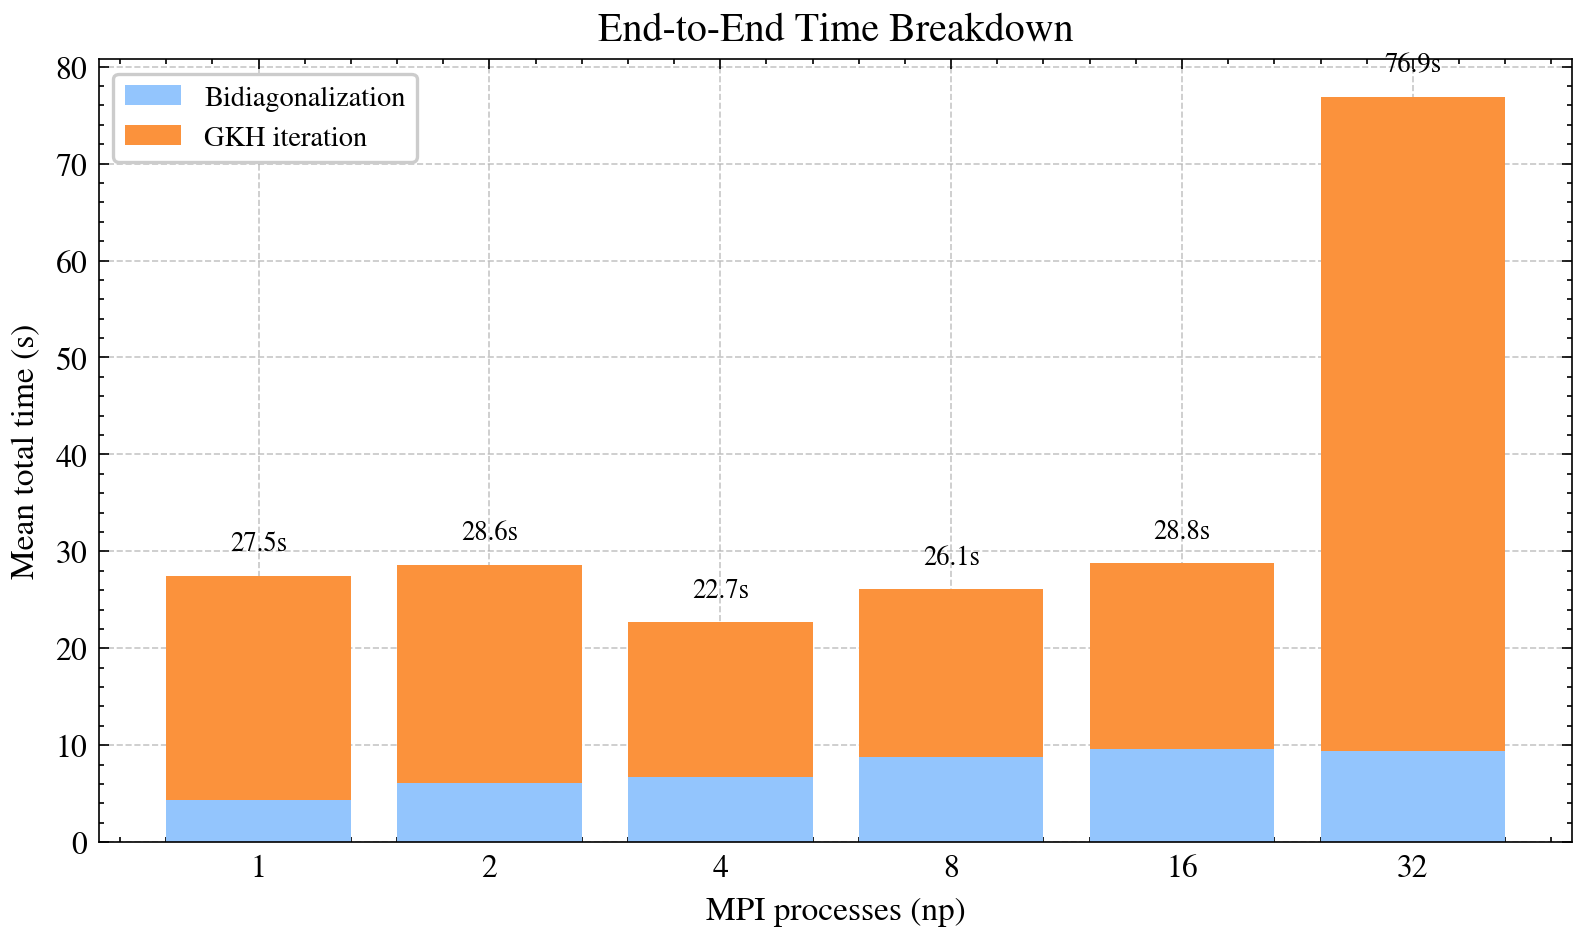
\includegraphics[width=0.78\textwidth]{figures/mpi_time_breakdown.png}
\caption{端到端时间构成}
\label{fig:mpi-breakdown}
\end{figure}

\subsection{基于计时数据的开销分析}
对 $1000\times1000$ 主测试样例而言，$U,B,V$ 三个矩阵各约含 $10^6$ 个 \texttt{double}，单矩阵约 8 MB，三者合计约 24 MB。由于 MPI 进程内存空间相互独立，每个 rank 都需要持有自己的矩阵副本；当进入并行分发轮次时，根进程还需要广播当前 $U,B,V$，这正是多进程 SVD 比多线程更难加速的核心原因之一。

结果回传虽然只传活动块相关数据，长度为 $k$ 的活动块回传量约为 $k^2+mk+nk$ 个 \texttt{double}，比完整矩阵小得多，但这种优化只有在活动块已经切分得比较小时才明显有效。如果迭代中长期只有一个大的非 $1\times1$ 活动块，任务池没有足够任务可分，程序会退回 0 号进程串行推进；如果强行让所有 worker 参与，则每轮广播 24 MB 级矩阵却只能处理少量有效任务，通信与复制成本会盖过计算收益。

表\ref{tab:scaling-real} 给出了这一现象的数据证据：$np=4$ 时 GKH 平均时间为 $15975.63$ ms，取得 1.45 倍 GKH 加速；继续增至 $np=8$ 后，GKH 时间回升到 $17322.33$ ms；跨节点 $np=16$ 为 $19177.90$ ms；$np=32$ 更退化到 $67490.93$ ms。若瓶颈只是计算量不足，增加进程数至少不应导致如此明显的退化；实际结果说明，复制、广播、结果合并和进程等待已经成为主要开销。$np=32$ 的 GKH 标准差约 36.5 秒，也说明高进程数下性能不仅更慢，而且更不稳定。

因此，本文的 profiling 结论是：当前实现中真正有收益的是中等进程数下对多个活动块的动态调度；当活动块数量不足或跨节点通信放大时，进程独立内存和全量矩阵同步会迅速抵消收益。

\subsection{编译优化等级影响}
表\ref{tab:opt-real} 和图\ref{fig:compiler-opt} 比较了 \texttt{-O0}、\texttt{-O1}、\texttt{-O2}、\texttt{-O3}。在固定 $np=8$ 和启用 SIMD 的情况下，\texttt{-O0} 总时间为 $121703.03$ ms；\texttt{-O1}、\texttt{-O2}、\texttt{-O3} 均将总时间降到约 25 秒，其中 \texttt{-O2} 最快，总加速比为 4.82。

\begin{table}[H]
\centering
\small
\begin{tabular}{lrrrr}
\toprule
优化等级 & 上二对角/ms & GKH/ms & 总时间/ms & 相对 O0 加速比\\
\midrule
\texttt{-O0} & 26995.80 & 94707.23 & 121703.03 & 1.00\\
\texttt{-O1} & 6727.19 & 19179.70 & 25906.89 & 4.70\\
\texttt{-O2} & 6203.41 & 19043.00 & 25246.41 & 4.82\\
\texttt{-O3} & 6030.14 & 19347.33 & 25377.48 & 4.80\\
\bottomrule
\end{tabular}
\caption{编译优化等级实验，固定 $np=8$、SIMD、种子 2412592，每组 3 次}
\label{tab:opt-real}
\end{table}

\begin{figure}[H]
\centering
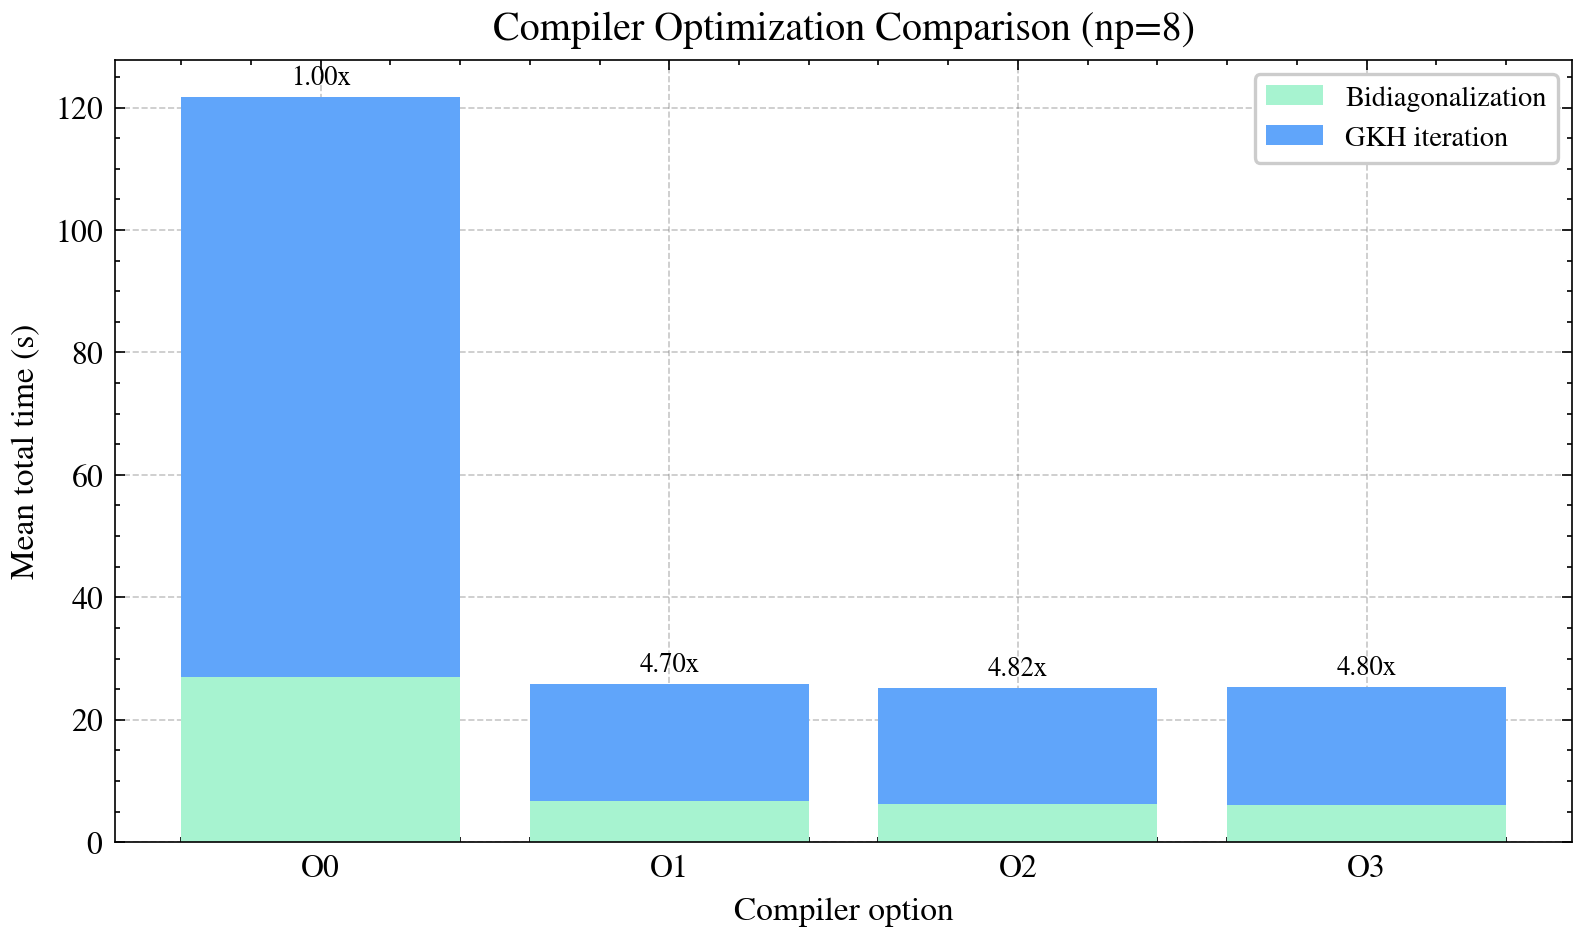
\includegraphics[width=0.78\textwidth]{figures/compiler_optimization.png}
\caption{编译优化等级对端到端耗时的影响}
\label{fig:compiler-opt}
\end{figure}

优化等级实验说明，编译器优化是本程序的基础性能条件。没有优化时，GKH 中大量循环、Givens 旋转和矩阵列更新会产生巨大开销；开启 \texttt{-O1} 后大部分收益已经出现，GKH 时间从 $94707.23$ ms 降到 $19179.70$ ms，约为原来的 20.3\%。\texttt{-O2} 相比 \texttt{-O1} 只继续减少约 3.5\% 的总时间，\texttt{-O3} 反而略慢于 \texttt{-O2}。这说明当前瓶颈并不只是单核浮点计算，调度、通信和内存访问也在限制性能。

这组数据还提醒我们不能把编译器优化收益误认为 MPI 收益。如果把 \texttt{-O0} 的结果和 \texttt{-O2} 的 MPI 结果直接比较，会得到非常大的“加速比”，但那主要来自编译器优化而不是并行任务池。因此后续规模扩展和 SIMD 对比均固定在 \texttt{-O2} 下进行。

\subsection{SIMD 与 MPI 的组合}
表\ref{tab:simd-real} 和图\ref{fig:simd} 给出 SIMD 开关对比。启用 SIMD 后，上二对角化平均耗时从 $10367.03$ ms 降至 $8232.26$ ms，加速约 1.26 倍；但 GKH 平均耗时从 $20227.73$ ms 变为 $20337.07$ ms，几乎没有提升，甚至略慢；总时间加速约 1.07 倍。

\begin{table}[H]
\centering
\small
\begin{tabular}{lrrrr}
\toprule
SIMD 设置 & 上二对角/ms & GKH/ms & 总时间/ms & 总时间标准差/ms\\
\midrule
启用 SIMD & 8232.26 & 20337.07 & 28569.33 & 2922.36\\
禁用 SIMD & 10367.03 & 20227.73 & 30594.76 & 2553.58\\
\bottomrule
\end{tabular}
\caption{SIMD 开关对比，固定 $np=8$、\texttt{-O2}、种子 2412592，每组 3 次}
\label{tab:simd-real}
\end{table}

\begin{figure}[H]
\centering
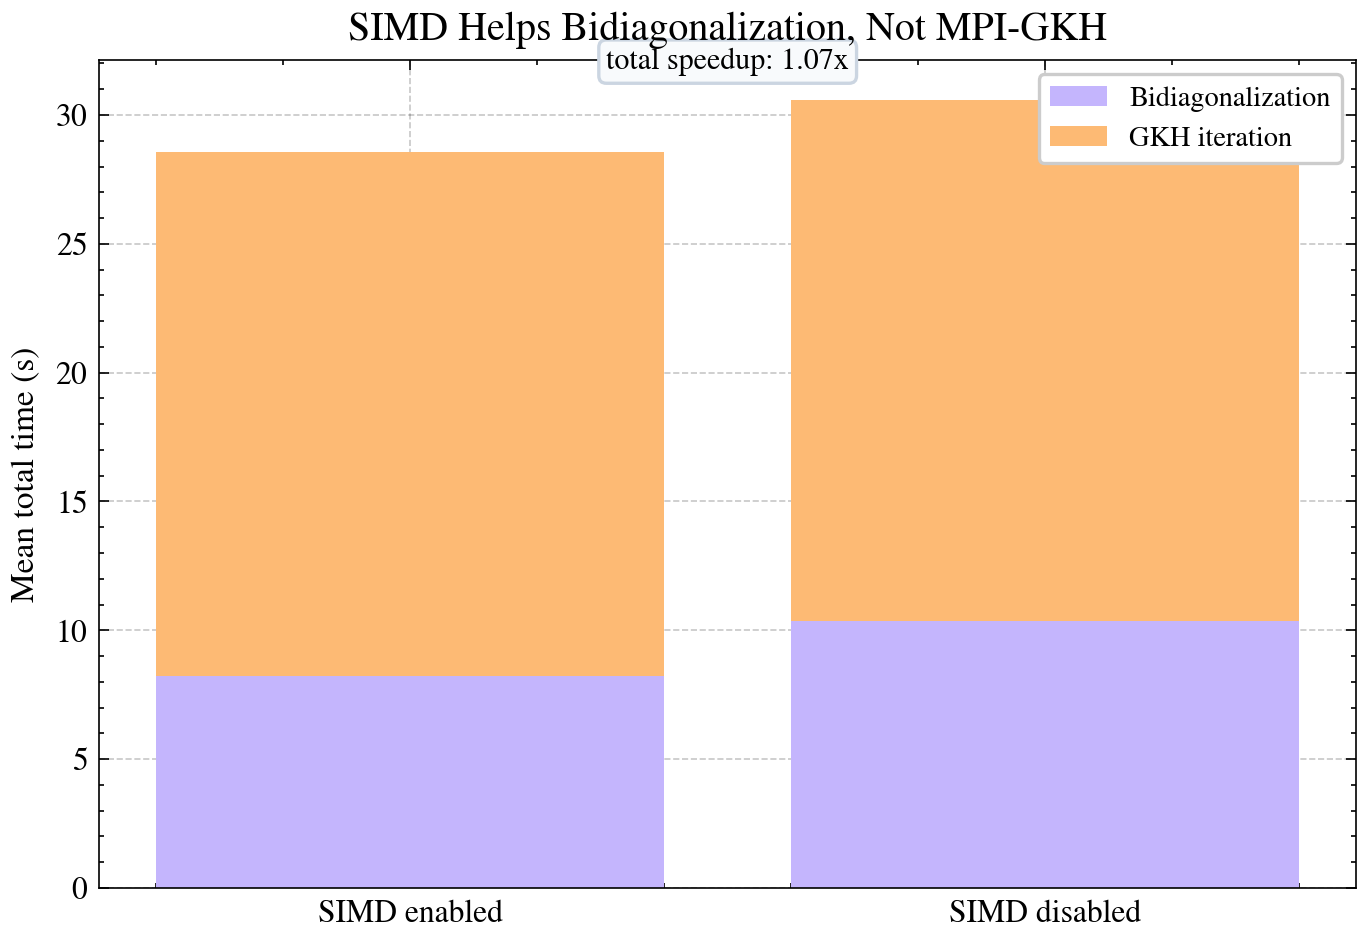
\includegraphics[width=0.70\textwidth]{figures/simd_comparison.png}
\caption{SIMD 开关对比}
\label{fig:simd}
\end{figure}

这组数据说明：MPI+SIMD 不一定优于只优化 SIMD，也不一定让 GKH 阶段明显变快。SIMD 主要加速连续向量运算，例如范数、点积和批量列更新；而本次 MPI-GKH 中，普通随机矩阵的瓶颈更多来自活动块并行度不足、矩阵广播、进程等待和结果合并。上二对角化阶段有较多连续向量计算，所以启用 SIMD 后从 $10367.03$ ms 降到 $8232.26$ ms；GKH 阶段虽然也有局部向量更新，但每轮还包含活动块扫描、shift 计算、Givens 参数生成和 MPI 同步，SIMD 覆盖比例较低，因此 $20337.07$ ms 与禁用 SIMD 的 $20227.73$ ms 基本处于实验波动范围内。

换言之，SIMD 优化提高的是单进程局部计算效率，而 MPI 任务池解决的是活动块级任务分发。两者不是简单相乘关系：当任务粒度足够大且通信相对较少时，SIMD 与 MPI 可以叠加；当通信和等待占主导时，SIMD 的局部收益会被更高层的并行开销吞没。

\subsection{重复运行稳定性}
为避免单次测量受队列状态和节点负载影响，固定 \texttt{-O2}+SIMD、$np=8$、种子 2412592 额外重复运行 5 次。结果见表\ref{tab:repeat-real} 和图\ref{fig:repeat}。总时间均值为 $26476.07$ ms，标准差为 $2110.68$ ms，变异系数为 8.0\%；GKH 变异系数为 9.3\%。

\begin{table}[H]
\centering
\small
\begin{tabular}{rrrr}
\toprule
重复次数 & 上二对角/ms & GKH/ms & 总时间变异系数\\
\midrule
5 & $6673.45 \pm 1354.86$ & $19802.62 \pm 1831.75$ & 8.0\%\\
\bottomrule
\end{tabular}
\caption{固定配置重复实验，\texttt{-O2}+SIMD、$np=8$、种子 2412592}
\label{tab:repeat-real}
\end{table}

\begin{figure}[H]
\centering
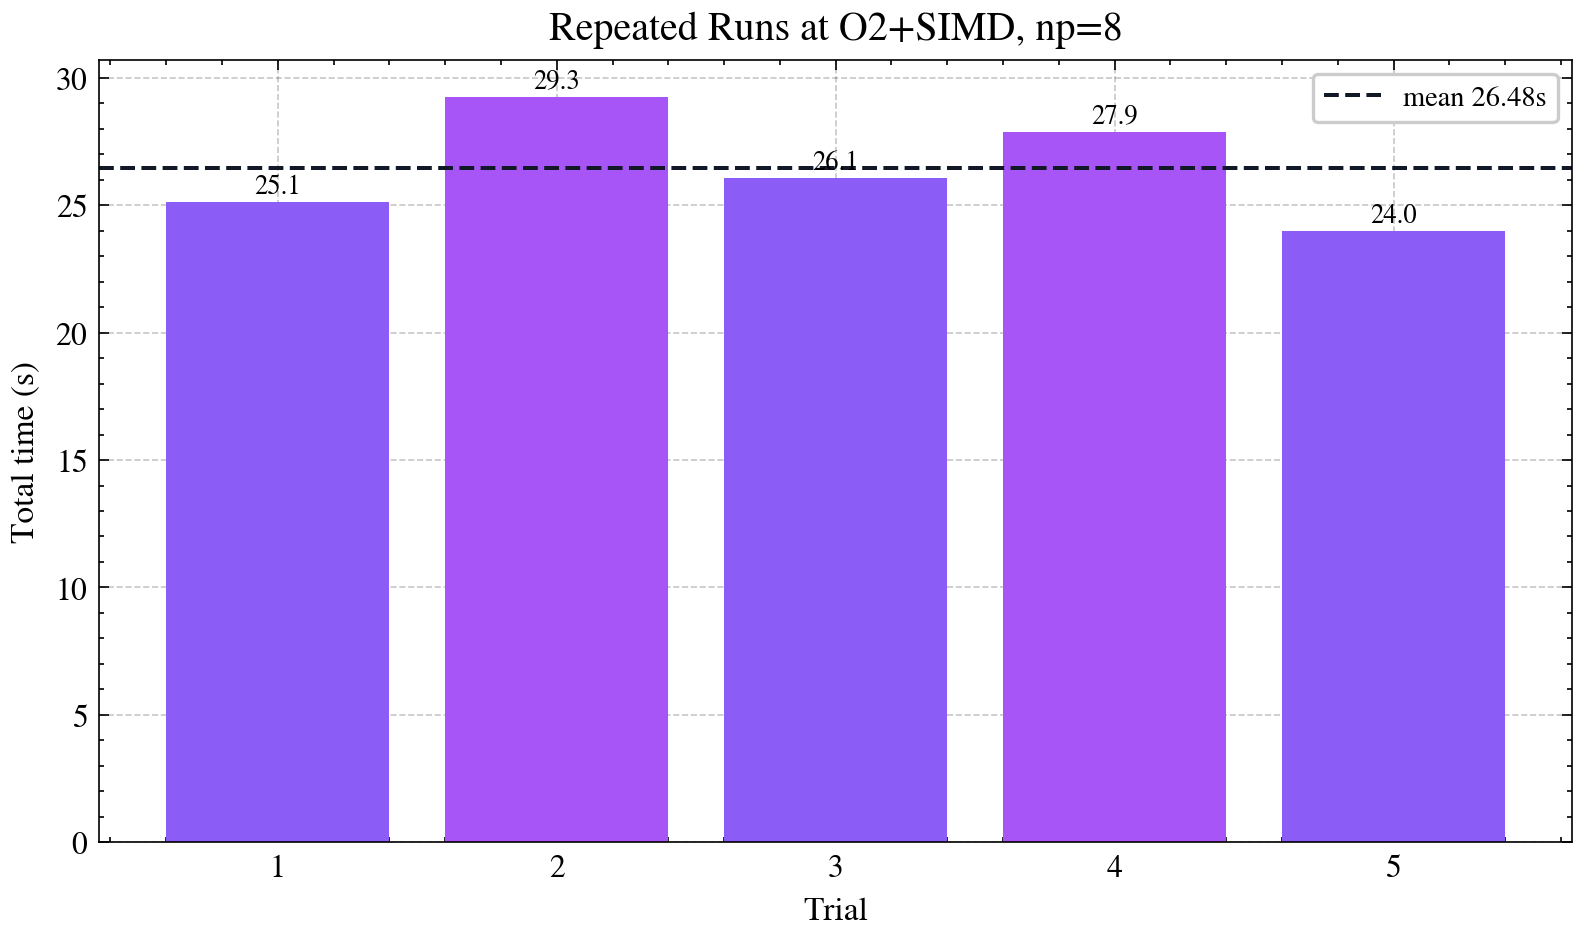
\includegraphics[width=0.78\textwidth]{figures/repeat_variability.png}
\caption{固定配置重复运行的总时间波动}
\label{fig:repeat}
\end{figure}

这说明服务器实验存在一定运行波动，尤其是 MPI 作业会受到节点分配、队列负载和跨节点通信状态影响。因此本文对规模扩展、优化等级和 SIMD 开关均使用多次重复的平均值，而不是选择单次最优结果。固定 $np=8$ 的重复实验中，总时间变异系数为 8.0\%，GKH 时间变异系数为 9.3\%，属于可以接受但不能忽略的波动范围。该处理也解释了部分表格中标准差较大的现象，例如 $np=32$ 的 GKH 标准差达到约 36.5 秒，说明过多进程不仅平均性能差，稳定性也更差。

因此，在评价本实验时，更有意义的不是某一次运行是否偶然较快，而是多次平均后是否呈现稳定趋势。规模扩展实验的趋势非常清楚：从 $np=1$ 到 $np=4$ 有有限加速，从 $np=8$ 开始收益下降，跨节点和高进程数下出现负优化。这一趋势与 SVD-GKH 活动块并行度有限的算法分析相一致。

\subsection{本地 VTune 热点 profiling}
在本地 Windows 环境中，使用 VTune 对 \texttt{-O2}、启用 SIMD、固定种子 2412592 的 \texttt{main.cpp} 单进程运行进行热点采样。该 profiling 不用于替代服务器 MPI 实验，因为它没有跨进程通信；它的作用是回答“每个进程内部主要把 CPU 时间花在哪里”。本地运行 5 个样例全部通过，最大规模 \texttt{1000x1000} 样例中，上二对角化耗时 $1935.63$ ms，GKH 耗时 $4129.38$ ms，总 GKH 耗时 $4239.91$ ms。

\begin{table}[H]
\centering
\small
\begin{tabular}{lrrl}
\toprule
热点函数 & CPU 时间/s & 占比 & 解释\\
\midrule
\texttt{apply\_right\_cols\_range} & 2.689 & 36.3\% & GKH 中对列区间应用右乘 Givens 更新\\
\texttt{Matrix::operator*} & 1.405 & 18.9\% & \texttt{main.cpp} 正确性验证中的矩阵重构乘法\\
\texttt{cleanup\_bidiagonal} & 0.618 & 8.3\% & 清理近零超对角元并划分活动块\\
\texttt{\_mm\_add\_pd} & 0.400 & 5.4\% & SIMD 双精度加法指令\\
\texttt{\_mm\_loadu\_pd} & 0.354 & 4.8\% & SIMD 非对齐加载指令\\
\texttt{simd\_dot} & 0.275 & 3.7\% & 上二对角化中的向量点积\\
\bottomrule
\end{tabular}
\caption{本地 VTune hotspots 结果，官方 \texttt{main.cpp} 单进程运行}
\label{tab:vtune-hotspots}
\end{table}

\begin{figure}[H]
\centering
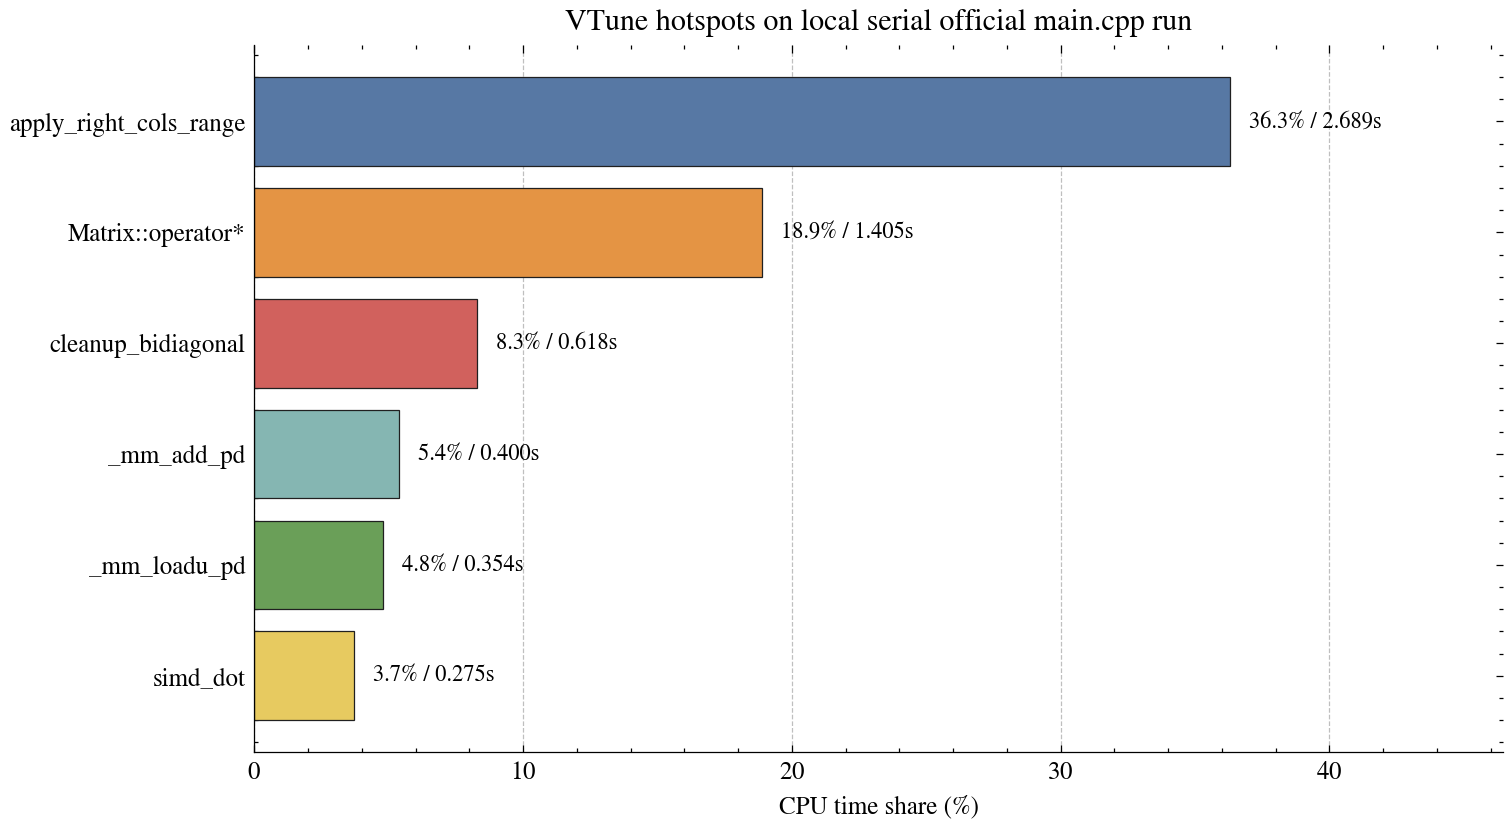
\includegraphics[width=0.78\textwidth]{figures/vtune_hotspots.png}
\caption{本地 VTune 热点函数占比}
\label{fig:vtune-hotspots}
\end{figure}

表\ref{tab:vtune-hotspots} 和图\ref{fig:vtune-hotspots} 表明，子进程内部最主要的热点是 GKH 的列区间更新函数 \texttt{apply\_right\_cols\_range}，占 CPU 时间 36.3\%。这与算法分析一致：bulge chasing 每一步都需要对 $B$ 和 $V$ 的相关列做 Givens 旋转，虽然局部操作可以被 SIMD 化，但访问模式和迭代依赖仍然决定了它是 GKH 的主要计算核。第二个热点 \texttt{Matrix::operator*} 来自 \texttt{main.cpp} 中的正确性验证，即计算 $U S V^T$ 的重构误差；它不属于被优化的 GKH 算法本体，但会出现在端到端时间和本地 profiling 中。

这一结果可以解释 SIMD 实验中的现象：VTune 的热点表中确实出现了 \texttt{\_mm\_add\_pd}、\texttt{\_mm\_loadu\_pd}、\texttt{simd\_dot} 等 SIMD 相关项，说明向量化代码被执行；但是在 MPI+GKH 场景中，活动块划分、清理、矩阵同步和任务等待共同参与耗时，所以 SIMD 指令热点并不能直接转化为 GKH 阶段的线性加速。也就是说，子进程内部仍有计算热点可优化，但服务器规模扩展曲线的主要限制已经上升到活动块并行度和 MPI 通信层面。

\section{进阶要求探索}

\subsection{不同平台与并行形态对比}
本实验主要运行平台是课程服务器，编译环境显示 MPI 头文件来自 \texttt{mpich-aarch64}，因此服务器数据可视为 ARM 平台上的 MPI+SIMD 实验。作为对照，本地 Windows x86 环境中保留了 serial、pthread 与 VTune profiling 数据。两类平台的 CPU、编译器、系统负载和矩阵规模并不完全一致，所以本文不把它们的绝对耗时直接横向比较，而只比较“同一平台、同一输入内部”的加速趋势。

\begin{table}[H]
\centering
\scriptsize
\begin{tabular}{llp{0.25\textwidth}rrr}
\toprule
平台 & 并行形态 & 代表样例 & GKH/ms & 加速比 & 可并行轮次\\
\midrule
x86 本地 & serial+SIMD & 随机 $512\times512$ & 4421.59 & 1.00 & --\\
x86 本地 & pthread4+SIMD & 随机 $512\times512$ & 4402.29 & 1.00 & $8/749$\\
x86 本地 & OpenMP4+SIMD & 随机 $512\times512$ & 4385.86 & 1.01 & $8/749$\\
x86 本地 & serial+SIMD & 4 个 $128$ 块 & 1130.35 & 1.00 & --\\
x86 本地 & pthread4+SIMD & 4 个 $128$ 块 & 360.63 & 3.13 & $252/253$\\
x86 本地 & OpenMP4+SIMD & 4 个 $128$ 块 & 359.08 & 3.15 & $252/253$\\
ARM 服务器 & MPI+SIMD, $np=1$ & 随机 $1000\times1000$ & 23147.60 & 1.00 & 未输出\\
ARM 服务器 & MPI+SIMD, $np=4$ & 随机 $1000\times1000$ & 15975.63 & 1.45 & 未输出\\
ARM 服务器 & MPI+SIMD, $np=32$ & 随机 $1000\times1000$ & 67490.93 & 0.34 & 未输出\\
\bottomrule
\end{tabular}
\caption{不同平台和并行形态的实测数据对比}
\label{tab:advanced-platform}
\end{table}

\begin{figure}[H]
\centering
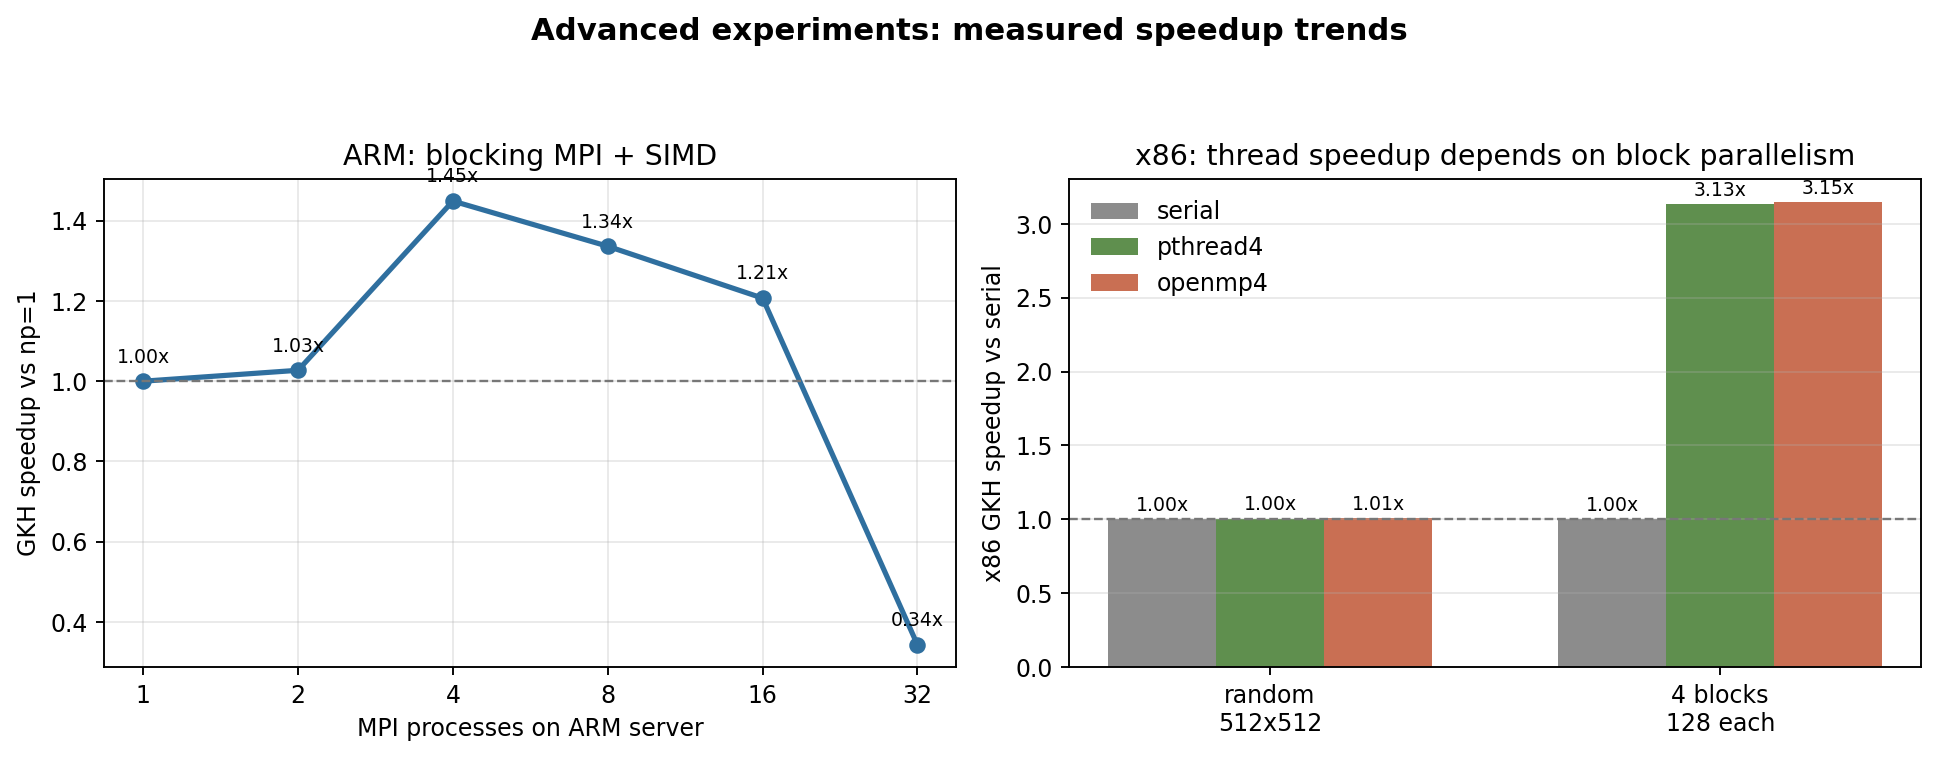
\includegraphics[width=0.92\textwidth]{figures/advanced_parallel_comparison.png}
\caption{不同平台与并行形态的相对加速趋势}
\label{fig:advanced-platform}
\end{figure}

本地补充实测在 Windows x86\_64 环境中完成，编译器为 MinGW-W64 \texttt{g++ 7.3.0}。这组实验不用于和 ARM 服务器做绝对耗时排名，而是固定同一平台、同一输入，比较 serial、pthread4 与 OpenMP4 在活动块并行度不同的情况下能否加速。OpenMP4 版本的编译与运行命令如下，随机种子固定为 20260408：

\begin{lstlisting}[language=bash]
g++ -std=c++17 -O2 -fopenmp experiment_driver.cpp \
    bidiagonalization.cpp gkh.cpp \
    -o profiling/experiment_openmp.exe

$env:SVD_MODE='openmp'
$env:SVD_THREADS='4'
.\profiling\experiment_openmp.exe --seed 20260408 --repeat 1 \
    --sizes 512x512 --gkh-blocks 128x4
\end{lstlisting}

实测输出中两个样例均为 \texttt{PASS}。随机 $512\times512$ 的相对重构误差为 $3.7935\times10^{-13}$，OpenMP4 的 GKH 时间为 4385.86 ms；4 个 $128$ 块结构样例的相对重构误差为 $3.8720\times10^{-13}$，OpenMP4 的 GKH 时间为 359.08 ms。与同一输入下的 serial 和 pthread4 数据放在一起可以看到：随机矩阵中 OpenMP4 只比 serial 快约 1.01 倍，而块结构中 OpenMP4 可达到 3.15 倍。这说明本地实测的核心变量不是“线程 API 名称”，而是活动块是否真的提供了足够的并行任务。

\begin{figure}[H]
\centering
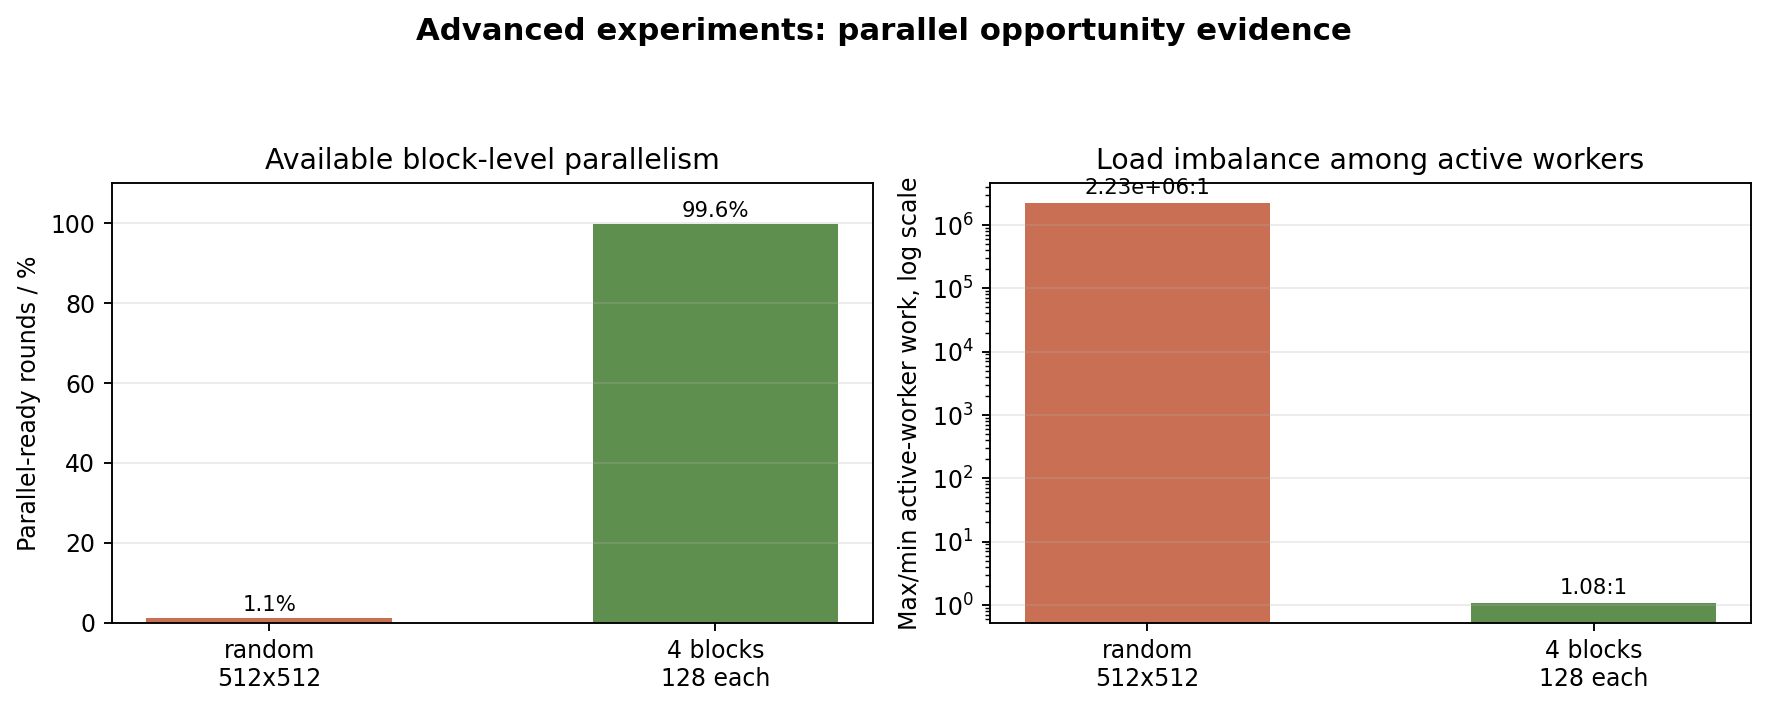
\includegraphics[width=0.86\textwidth]{figures/parallel_opportunity_evidence.png}
\caption{活动块并行机会与工作量不均衡}
\label{fig:parallel-opportunity}
\end{figure}

表\ref{tab:advanced-platform}、图\ref{fig:advanced-platform} 和图\ref{fig:parallel-opportunity} 的关键结论是：平台差异不是唯一决定因素，活动块并行度更直接决定了并行收益。本地 x86 上，随机 $512\times512$ 的可并行轮次只有 $8/749$，pthread4 和 OpenMP4 的 GKH 加速比分别只有 1.00 和 1.01；同时 active worker 的最大/最小工作量比例约为 $2.23\times10^6:1$，说明几乎所有实质工作仍集中在一个 worker 上。相反，4 个 $128$ 块样例中可并行轮次为 $252/253$，最大/最小工作量比例仅约 $1.08:1$，pthread4 和 OpenMP4 分别达到 3.13 和 3.15 倍加速。ARM 服务器上也呈现类似趋势：当 $np=4$ 仍能承接一定活动块时，MPI+SIMD 有有限收益；当 $np=32$ 远大于可同时处理的活动块数量时，通信和等待开销超过计算收益，性能显著退化。

这组进阶对比说明，多线程、SIMD 和 MPI 的关系不是简单叠加。SIMD 改善单个 rank 或线程内部的向量运算，多线程和 MPI 需要足够多的独立任务才能发挥作用。若算法长期只有一个大活动块，换成更多线程、更多进程或更强平台都难以自动获得线性加速。

\subsection{不同 MPI 编程方法的比较}
本次最终代码采用阻塞双边通信：根进程通过 \texttt{MPI\_Bcast} 同步矩阵状态，通过 \texttt{MPI\_Send}/\texttt{MPI\_Recv} 下发任务和回收结果，并使用 \texttt{MPI\_ANY\_SOURCE} 实现动态任务领取。选择该方案的原因是它最容易保证 GKH 每轮矩阵状态一致，也便于定位正确性问题。表\ref{tab:mpi-methods} 总结了可选 MPI 编程方法在本 SVD-GKH 场景中的适用性。

\begin{table}[H]
\centering
\small
\begin{tabular}{p{0.18\textwidth}p{0.24\textwidth}p{0.25\textwidth}p{0.23\textwidth}}
\toprule
方法 & 适用点 & 可能收益 & 主要风险\\
\midrule
阻塞双边通信 & 已在最终代码中实现，任务和结果顺序清晰 & 正确性最稳定，便于统计广播与回传开销 & 根进程等待明显，通信与计算重叠少\\
非阻塞双边通信 & 可将 \texttt{MPI\_Isend}/\texttt{MPI\_Irecv} 用于任务下发和结果回收 & 当 ready task 很多时，有机会隐藏部分结果回传延迟 & GKH 下一轮依赖合并后的矩阵状态，普通随机矩阵中可重叠空间有限\\
单边通信 RMA & 可尝试用 \texttt{MPI\_Win} 暴露活动块缓冲区，由 worker 主动读写 & 理论上减少根进程参与频率，适合固定缓冲区反复复用 & 一致性、锁和窗口同步复杂；$U,V$ 列更新不连续，容易引入合并错误\\
MPI 自身多线程支持 & 可用 \texttt{MPI\_Init\_thread} 组成 MPI+pthread 混合模型 & 一节点一个或少量 rank，rank 内用线程，可减少跨进程矩阵复制 & \texttt{MPI\_THREAD\_MULTIPLE} 可能带来额外锁开销；需要严格限定通信线程\\
\bottomrule
\end{tabular}
\caption{不同 MPI 编程方法在 SVD-GKH 中的适用性分析}
\label{tab:mpi-methods}
\end{table}

\begin{table}[H]
\centering
\small
\begin{tabular}{rrrr}
\toprule
$np$ & 每轮完整 $U+B+V$ 广播量/MB & GKH 平均耗时/ms & GKH 加速比\\
\midrule
1 & 0 & 23147.60 & 1.00\\
2 & 24 & 22535.20 & 1.03\\
4 & 72 & 15975.63 & 1.45\\
8 & 168 & 17322.33 & 1.34\\
16 & 360 & 19177.90 & 1.21\\
32 & 744 & 67490.93 & 0.34\\
\bottomrule
\end{tabular}
\caption{阻塞 MPI 方案的通信量估算与实测性能}
\label{tab:mpi-comm-evidence}
\end{table}

从当前 41 组服务器数据和表\ref{tab:mpi-comm-evidence} 看，最值得继续尝试的不是盲目引入更复杂的通信模型，而是混合并行：节点间使用较少 MPI rank，节点内复用已有 pthread/OpenMP 活动块任务池。对 $1000\times1000$ 主样例，$U,B,V$ 三个矩阵合计约 24 MB；当前阻塞方案每次进入分发轮次都要向 $world\_size-1$ 个 worker 广播完整矩阵，因此 $np=32$ 时单轮广播量估计达到 744 MB。非阻塞通信可以隐藏一部分发送/接收等待，但不能减少这部分数据量；单边通信也仍需处理同样的矩阵一致性问题。结合图\ref{fig:parallel-opportunity} 中随机矩阵只有 1.07\% 的可并行轮次，非阻塞和单边通信在普通随机矩阵上能重叠的计算窗口很小，更适合作为有块结构输入或混合并行方案上的后续优化分支。

\subsection{其他算法优化策略}
除通信方式外，本实验还可以从算法层面继续优化。第一，设置任务粒度阈值：当活动块数量少或块太小时，直接在根进程串行推进，避免广播完整矩阵。当前实现已经包含“只有一个非平凡块时串行推进”的思想，后续可把阈值从数量扩展到估算工作量。第二，减少同步数据量：不要每轮广播完整 $U,B,V$，而是只同步与活动块相关的 $B$ 子块和 $U,V$ 列区间；这一策略能够直接降低表\ref{tab:mpi-methods} 中阻塞通信的主要开销。第三，延迟更新正交矩阵：先记录 Givens 旋转序列，待若干轮后批量更新 $U,V$，可能提升缓存局部性和 SIMD 覆盖率，但需要额外验证重构误差和数值稳定性。第四，构造并识别块结构输入：本地 x86 的 4 块样例说明，只要活动块数量充足，已有任务池就能取得明显收益；因此对具有块结构或近似块对角结构的矩阵，MPI 任务池更可能发挥作用。

\section{综合讨论}

\subsection{为什么 $np=4$ 最优}
从实验结果看，$np=4$ 是当前实现和测试数据上的最佳折中。它仍然位于单节点内，通信主要是节点内 MPI 通信，广播和回收开销较低；同时相比 $np=1$ 和 $np=2$，它又有足够进程承接 deflation 后出现的多个活动块。继续增加到 $np=8$ 后，并行度增长已经赶不上调度和等待成本；跨节点的 $np=16$、$np=32$ 则进一步放大了数据复制和通信开销。

这说明本实验的性能瓶颈不是“没有 MPI”，而是 SVD-GKH 本身很难在普通随机矩阵上长期提供大量独立任务。实验手册中的特殊情况说明也指出，迭代中可能长期只有一个非 $1\times1$ 大矩阵，其余矩阵都已经收敛；本实验的规模扩展曲线正体现了这一性质。

\subsection{MPI 任务池的价值与限制}
任务池的价值在于正确处理了负载不均衡问题：当多个活动块存在时，工作进程不是静态绑定某个块，而是空闲后继续领取任务。这比固定块划分更适合 GKH 中块大小不断变化的过程。但任务池不能创造算法并行度。如果某一轮只有一个大活动块，根进程串行推进反而是更优选择，因为强行广播完整矩阵只会增加开销。

因此，当前实现对“块数量足够”的场景是有效的，对普通随机矩阵只能获得有限收益。后续如果要进一步优化，可以考虑两条方向：一是寻找活动块内部更细粒度但数学上安全的并行更新；二是减少广播量，例如只同步与当前活动块相关的矩阵列，或在多轮任务之间复用工作进程状态，避免每次都广播完整 $U,B,V$。

\subsection{与前序 SIMD 实验的关系}
SIMD 优化仍然是必要的基础优化。它对上二对角化阶段有稳定收益，并能降低局部向量运算成本。但在 MPI-GKH 中，SIMD 无法解决进程等待、活动块数量不足和通信放大问题。因此不能简单地说“MPI+SIMD 一定最快”。更准确的结论是：SIMD 提高单进程计算核效率，MPI 提供跨进程任务调度能力；只有当任务粒度足够大、通信足够少、活动块足够多时，二者叠加才可能得到明显收益。

\section{总结}
本次实验完成了 SVD 算子的 MPI 并行化实现和服务器实验验证。代码层面将 MPI 初始化和任务池逻辑封装在 \texttt{gkh.cpp} 中；实验流程层面按照修正脚本说明，使用 \texttt{mpic++} 编译和 \texttt{qsub\_mpi.sh} 提交。

从 41 组真实服务器数据看，程序正确性稳定，全部测试通过，误差保持在 $10^{-13}$ 量级。性能方面，GKH 阶段在 $np=4$ 时取得最好平均结果，加速比为 1.45；$np=8$ 后收益下降，$np=32$ 出现明显负优化。编译优化对性能影响显著，\texttt{-O2} 相比 \texttt{-O0} 端到端加速 4.82 倍；SIMD 对上二对角化有 1.26 倍收益，但对 MPI-GKH 基本无提升。综合来看，SVD 的 MPI 加速受活动块并行度强烈限制，任务池实现是必要的，但通信和算法粒度决定了其上限。

进阶探索部分进一步对比了 ARM 服务器 MPI+SIMD 与本地 x86 pthread/OpenMP+SIMD 的趋势。结果表明，随机矩阵的可并行轮次只有 $8/749$，pthread4 和 OpenMP4 都只能获得约 1.0 倍 GKH 加速；人工块结构样例的可并行轮次达到 $252/253$，pthread4 与 OpenMP4 分别达到 3.13 和 3.15 倍 GKH 加速。MPI 通信量估算也显示，$np=32$ 时完整 $U+B+V$ 广播量每轮可达约 744 MB。这说明后续优化的重点应放在减少通信复制、提高活动块并行度以及发展 MPI+线程的混合并行，而不是单纯增加进程数。


\newpage
\section*{附录 A：生成式 AI 辅助学习对话记录}
\addcontentsline{toc}{section}{附录 A：生成式 AI 辅助学习对话记录}

本附录记录了实验过程中利用生成式 AI 辅助理解 SIMD、多线程和 MPI 编程的对话截图。提问方式遵循“先给出自己的实现、实验数据或瓶颈判断，再请求 AI 检查和分析”的原则，避免直接要求 AI 代写完整代码或编造实验结论。

\begin{figure}[H]
\centering
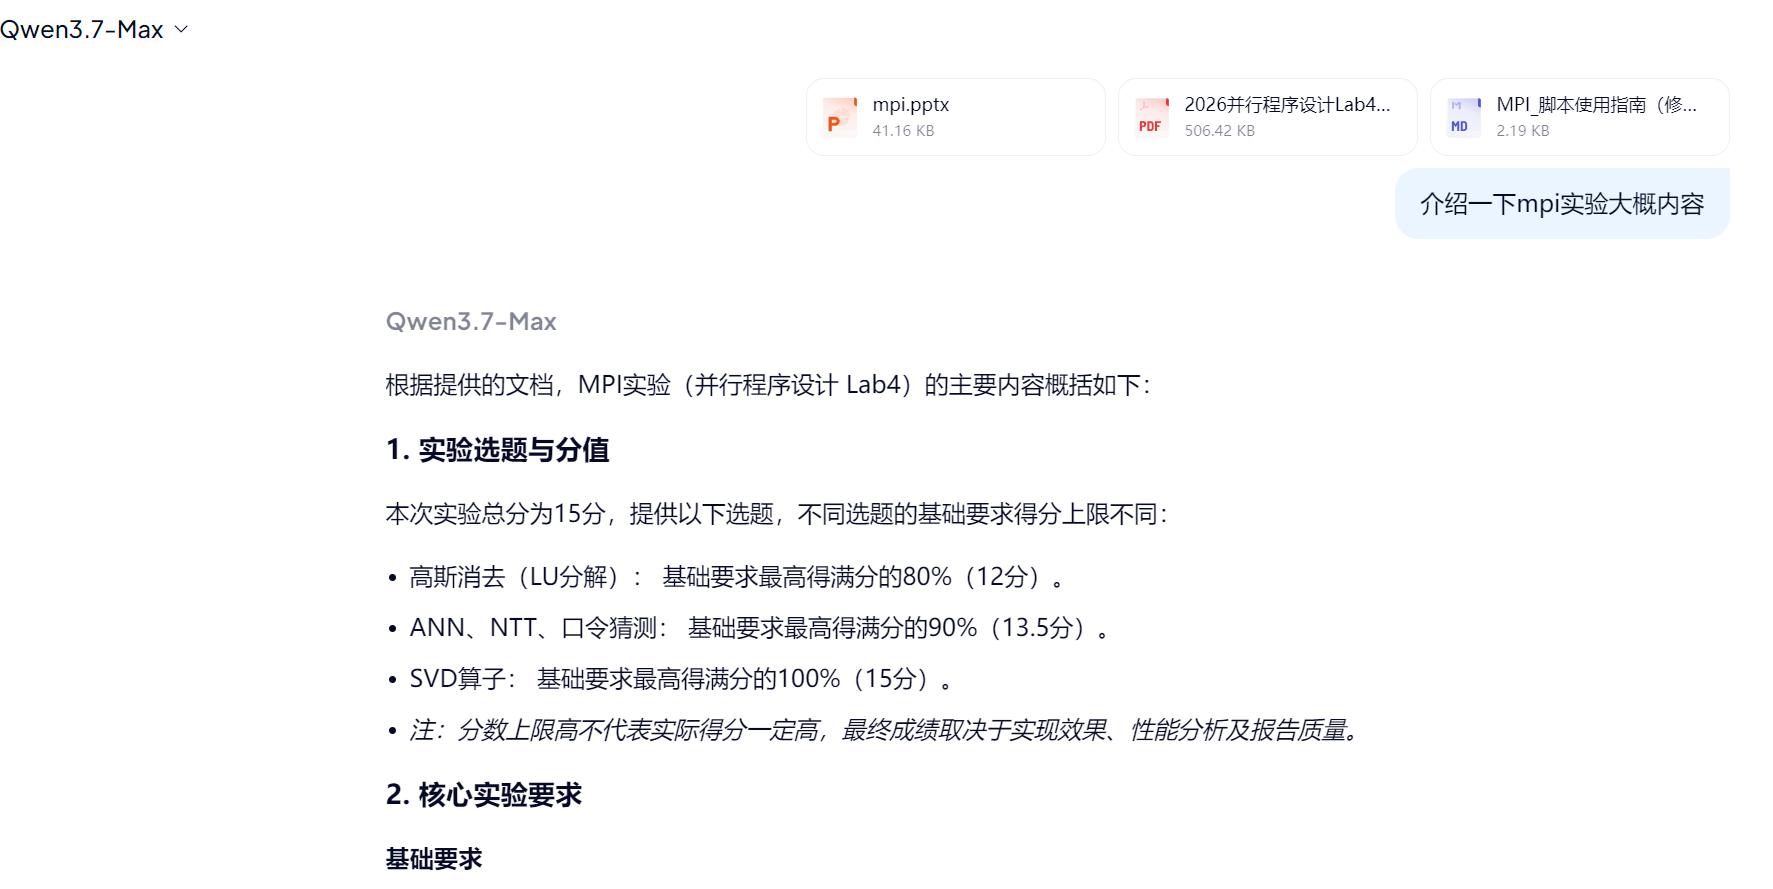
\includegraphics[width=0.96\textwidth,height=0.78\textheight,keepaspectratio]{figures/ai_dialog_q1.png}
\caption{AI 辅助学习对话记录 1}
\label{fig:ai-dialog-q1}
\end{figure}

\begin{figure}[H]
\centering
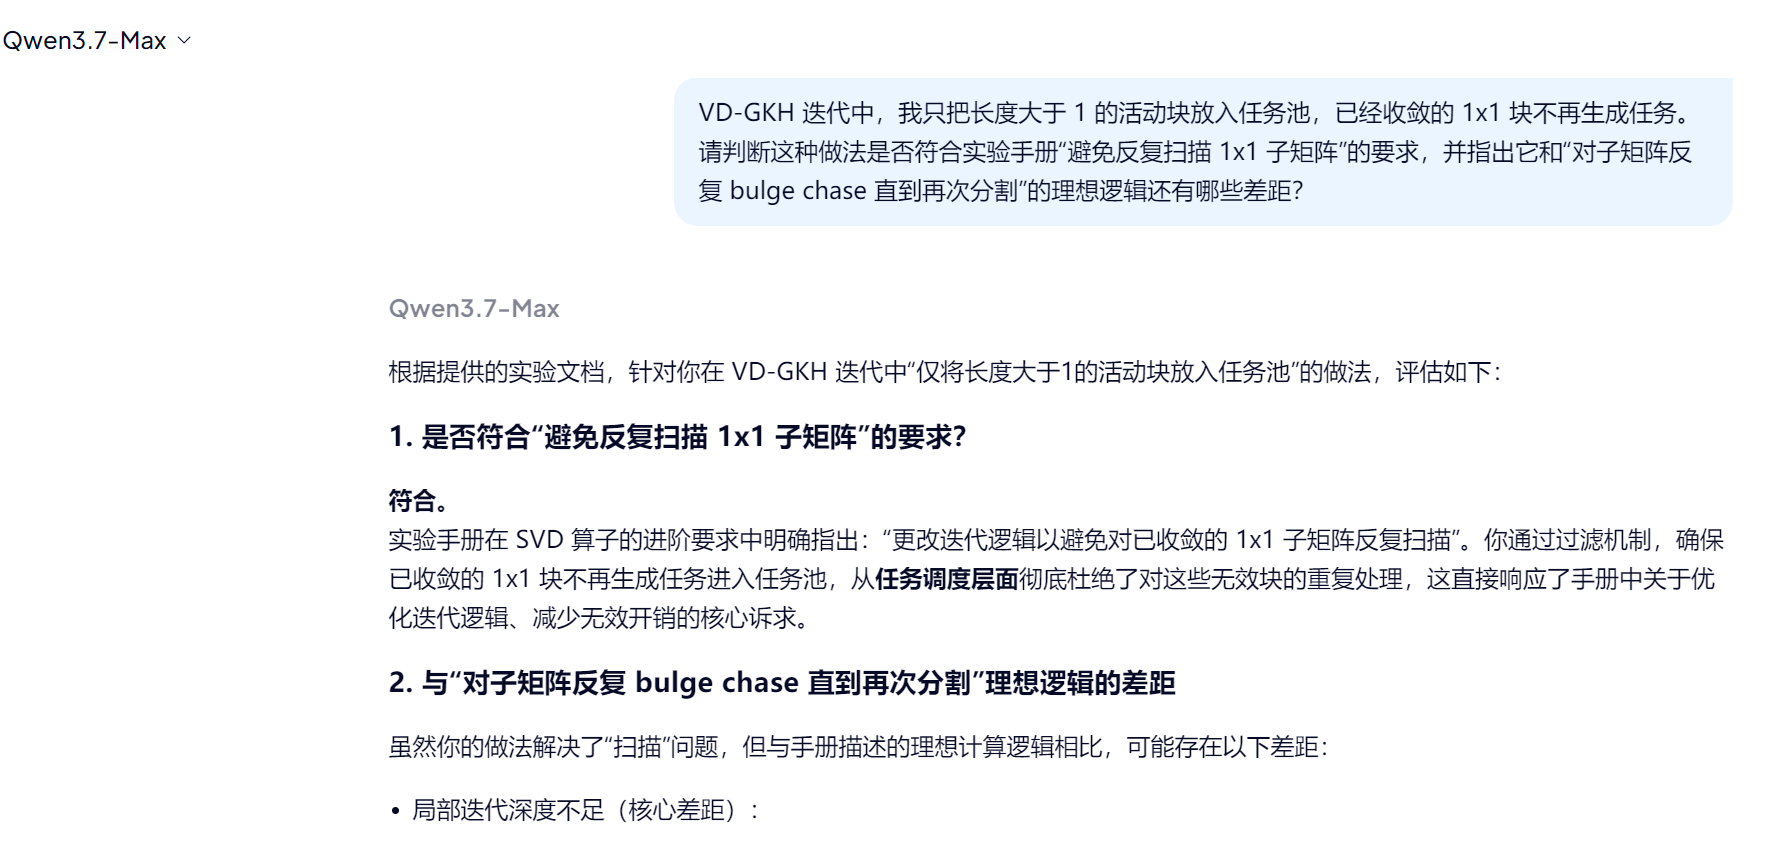
\includegraphics[width=0.96\textwidth,height=0.78\textheight,keepaspectratio]{figures/ai_dialog_q2.png}
\caption{AI 辅助学习对话记录 2}
\label{fig:ai-dialog-q2}
\end{figure}

\begin{figure}[H]
\centering
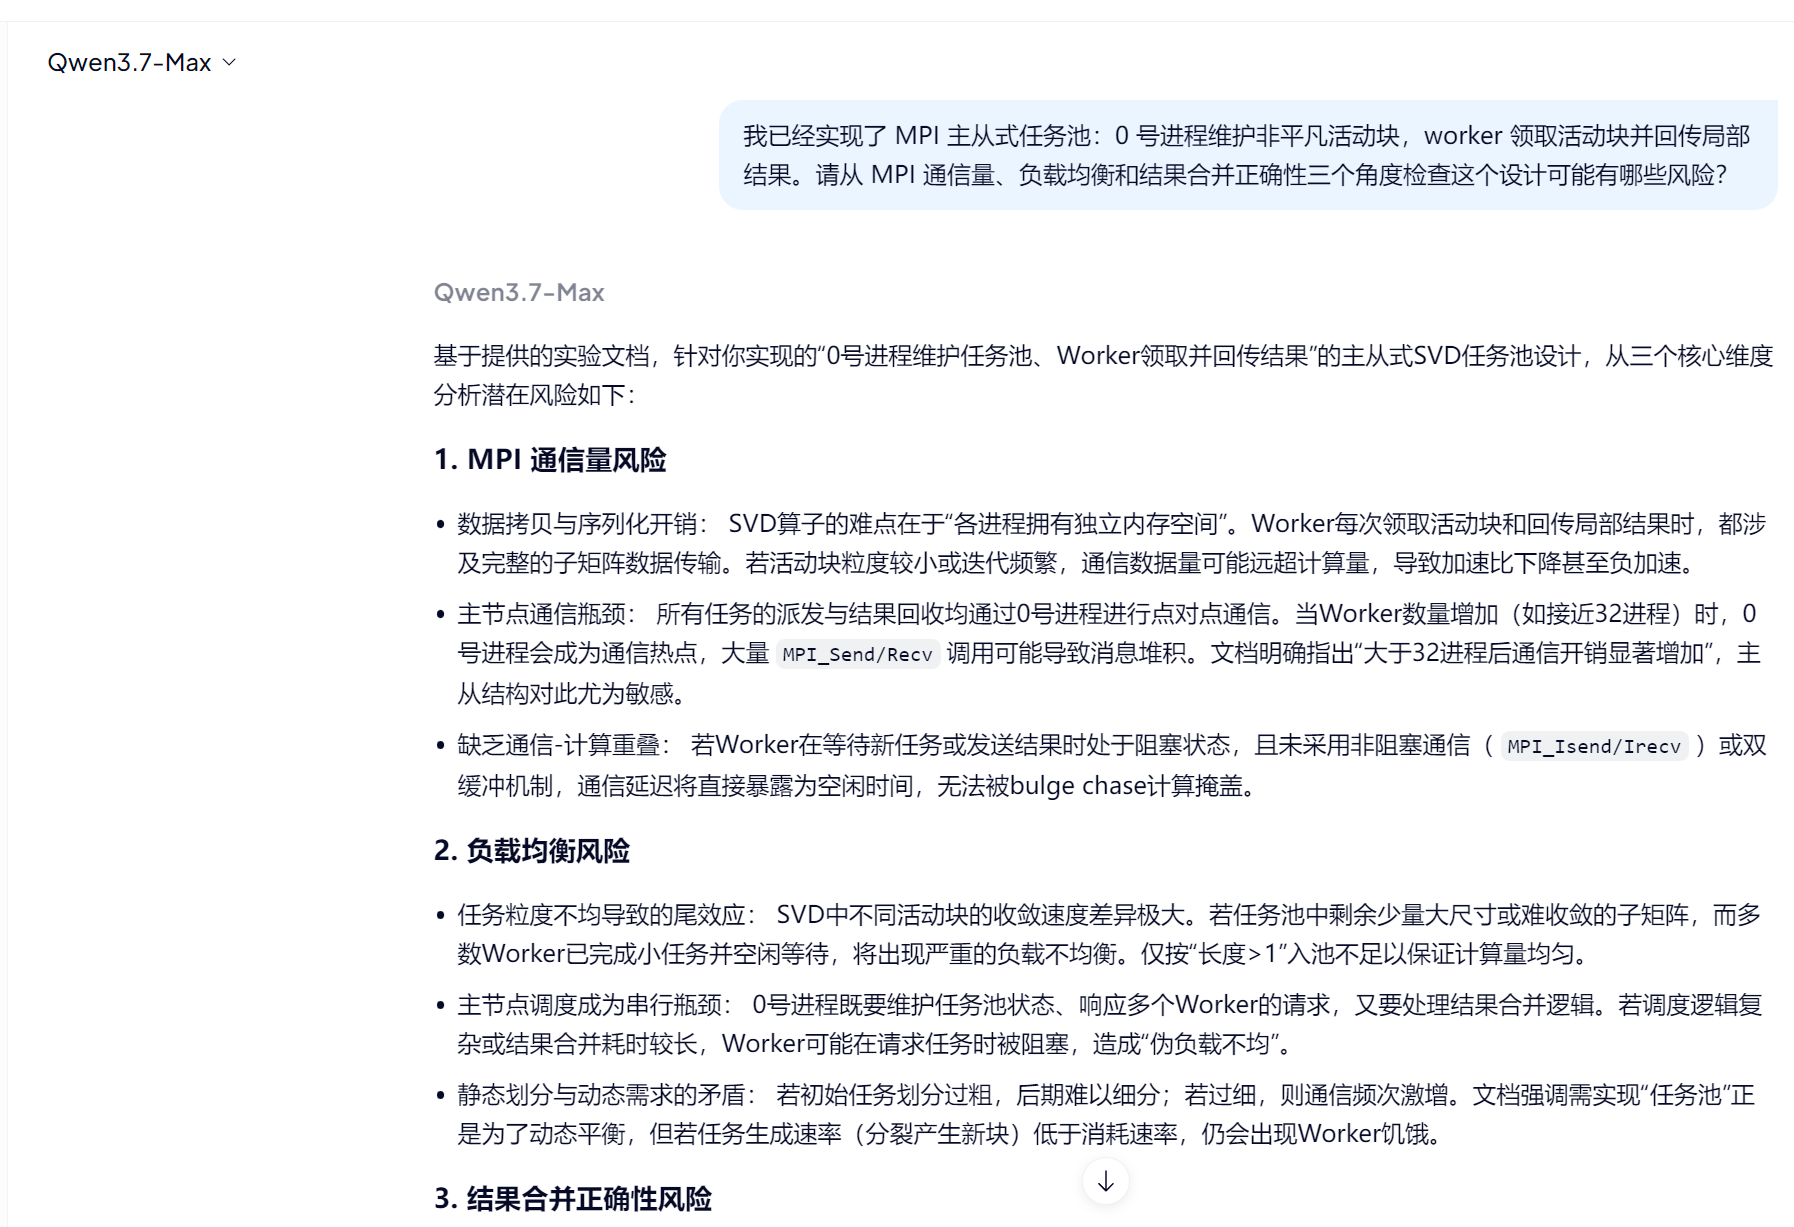
\includegraphics[width=0.96\textwidth,height=0.78\textheight,keepaspectratio]{figures/ai_dialog_q3.png}
\caption{AI 辅助学习对话记录 3}
\label{fig:ai-dialog-q3}
\end{figure}

\begin{figure}[H]
\centering
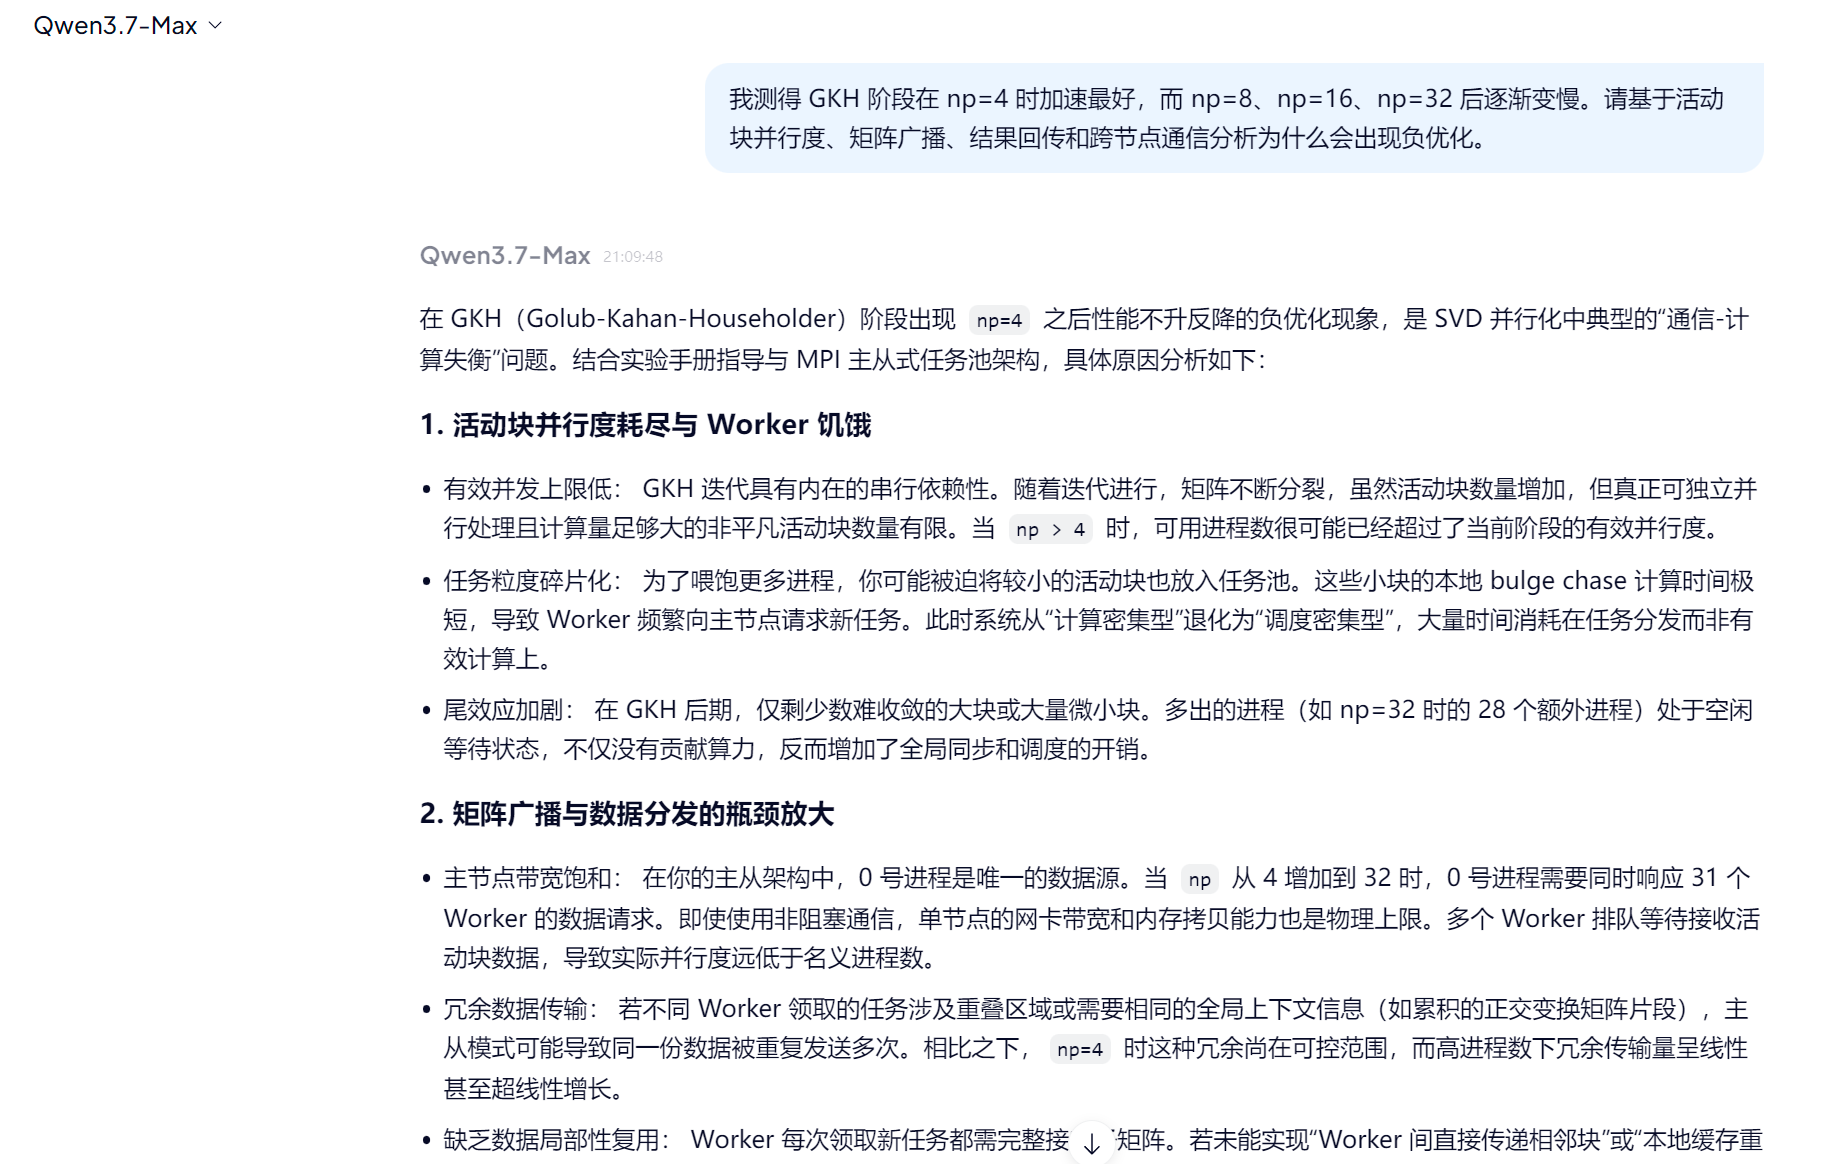
\includegraphics[width=0.96\textwidth,height=0.78\textheight,keepaspectratio]{figures/ai_dialog_q4.png}
\caption{AI 辅助学习对话记录 4}
\label{fig:ai-dialog-q4}
\end{figure}

\newpage
\bibliographystyle{plain}
\bibliography{references}

\end{document}
